\documentclass[11pt]{article}

    \usepackage[breakable]{tcolorbox}
    \usepackage{parskip} % Stop auto-indenting (to mimic markdown behaviour)
    
    \usepackage{fontspec, xunicode, xltxtra}
    \setmainfont{Microsoft YaHei}
    \usepackage{ctex}

    \usepackage{iftex}
    \ifPDFTeX


    	\usepackage[T1]{fontenc}
    	\usepackage{mathpazo}
    \else
    	\usepackage{fontspec}
    \fi

    % Basic figure setup, for now with no caption control since it's done
    % automatically by Pandoc (which extracts ![](path) syntax from Markdown).
    \usepackage{graphicx}
    % Maintain compatibility with old templates. Remove in nbconvert 6.0
    \let\Oldincludegraphics\includegraphics
    % Ensure that by default, figures have no caption (until we provide a
    % proper Figure object with a Caption API and a way to capture that
    % in the conversion process - todo).
    \usepackage{caption}
    \DeclareCaptionFormat{nocaption}{}
    \captionsetup{format=nocaption,aboveskip=0pt,belowskip=0pt}

    \usepackage[Export]{adjustbox} % Used to constrain images to a maximum size
    \adjustboxset{max size={0.9\linewidth}{0.9\paperheight}}
    \usepackage{float}
    \floatplacement{figure}{H} % forces figures to be placed at the correct location
    \usepackage{xcolor} % Allow colors to be defined
    \usepackage{enumerate} % Needed for markdown enumerations to work
    \usepackage{geometry} % Used to adjust the document margins
    \usepackage{amsmath} % Equations
    \usepackage{amssymb} % Equations
    \usepackage{textcomp} % defines textquotesingle
    % Hack from http://tex.stackexchange.com/a/47451/13684:
    \AtBeginDocument{%
        \def\PYZsq{\textquotesingle}% Upright quotes in Pygmentized code
    }
    \usepackage{upquote} % Upright quotes for verbatim code
    \usepackage{eurosym} % defines \euro
    \usepackage[mathletters]{ucs} % Extended unicode (utf-8) support
    \usepackage{fancyvrb} % verbatim replacement that allows latex
    \usepackage{grffile} % extends the file name processing of package graphics 
                         % to support a larger range
    \makeatletter % fix for grffile with XeLaTeX
    \def\Gread@@xetex#1{%
      \IfFileExists{"\Gin@base".bb}%
      {\Gread@eps{\Gin@base.bb}}%
      {\Gread@@xetex@aux#1}%
    }
    \makeatother

    % The hyperref package gives us a pdf with properly built
    % internal navigation ('pdf bookmarks' for the table of contents,
    % internal cross-reference links, web links for URLs, etc.)
    \usepackage{hyperref}
    % The default LaTeX title has an obnoxious amount of whitespace. By default,
    % titling removes some of it. It also provides customization options.
    \usepackage{titling}
    \usepackage{longtable} % longtable support required by pandoc >1.10
    \usepackage{booktabs}  % table support for pandoc > 1.12.2
    \usepackage[inline]{enumitem} % IRkernel/repr support (it uses the enumerate* environment)
    \usepackage[normalem]{ulem} % ulem is needed to support strikethroughs (\sout)
                                % normalem makes italics be italics, not underlines
    \usepackage{mathrsfs}
    

    
    % Colors for the hyperref package
    \definecolor{urlcolor}{rgb}{0,.145,.698}
    \definecolor{linkcolor}{rgb}{.71,0.21,0.01}
    \definecolor{citecolor}{rgb}{.12,.54,.11}

    % ANSI colors
    \definecolor{ansi-black}{HTML}{3E424D}
    \definecolor{ansi-black-intense}{HTML}{282C36}
    \definecolor{ansi-red}{HTML}{E75C58}
    \definecolor{ansi-red-intense}{HTML}{B22B31}
    \definecolor{ansi-green}{HTML}{00A250}
    \definecolor{ansi-green-intense}{HTML}{007427}
    \definecolor{ansi-yellow}{HTML}{DDB62B}
    \definecolor{ansi-yellow-intense}{HTML}{B27D12}
    \definecolor{ansi-blue}{HTML}{208FFB}
    \definecolor{ansi-blue-intense}{HTML}{0065CA}
    \definecolor{ansi-magenta}{HTML}{D160C4}
    \definecolor{ansi-magenta-intense}{HTML}{A03196}
    \definecolor{ansi-cyan}{HTML}{60C6C8}
    \definecolor{ansi-cyan-intense}{HTML}{258F8F}
    \definecolor{ansi-white}{HTML}{C5C1B4}
    \definecolor{ansi-white-intense}{HTML}{A1A6B2}
    \definecolor{ansi-default-inverse-fg}{HTML}{FFFFFF}
    \definecolor{ansi-default-inverse-bg}{HTML}{000000}

    % commands and environments needed by pandoc snippets
    % extracted from the output of `pandoc -s`
    \providecommand{\tightlist}{%
      \setlength{\itemsep}{0pt}\setlength{\parskip}{0pt}}
    \DefineVerbatimEnvironment{Highlighting}{Verbatim}{commandchars=\\\{\}}
    % Add ',fontsize=\small' for more characters per line
    \newenvironment{Shaded}{}{}
    \newcommand{\KeywordTok}[1]{\textcolor[rgb]{0.00,0.44,0.13}{\textbf{{#1}}}}
    \newcommand{\DataTypeTok}[1]{\textcolor[rgb]{0.56,0.13,0.00}{{#1}}}
    \newcommand{\DecValTok}[1]{\textcolor[rgb]{0.25,0.63,0.44}{{#1}}}
    \newcommand{\BaseNTok}[1]{\textcolor[rgb]{0.25,0.63,0.44}{{#1}}}
    \newcommand{\FloatTok}[1]{\textcolor[rgb]{0.25,0.63,0.44}{{#1}}}
    \newcommand{\CharTok}[1]{\textcolor[rgb]{0.25,0.44,0.63}{{#1}}}
    \newcommand{\StringTok}[1]{\textcolor[rgb]{0.25,0.44,0.63}{{#1}}}
    \newcommand{\CommentTok}[1]{\textcolor[rgb]{0.38,0.63,0.69}{\textit{{#1}}}}
    \newcommand{\OtherTok}[1]{\textcolor[rgb]{0.00,0.44,0.13}{{#1}}}
    \newcommand{\AlertTok}[1]{\textcolor[rgb]{1.00,0.00,0.00}{\textbf{{#1}}}}
    \newcommand{\FunctionTok}[1]{\textcolor[rgb]{0.02,0.16,0.49}{{#1}}}
    \newcommand{\RegionMarkerTok}[1]{{#1}}
    \newcommand{\ErrorTok}[1]{\textcolor[rgb]{1.00,0.00,0.00}{\textbf{{#1}}}}
    \newcommand{\NormalTok}[1]{{#1}}
    
    % Additional commands for more recent versions of Pandoc
    \newcommand{\ConstantTok}[1]{\textcolor[rgb]{0.53,0.00,0.00}{{#1}}}
    \newcommand{\SpecialCharTok}[1]{\textcolor[rgb]{0.25,0.44,0.63}{{#1}}}
    \newcommand{\VerbatimStringTok}[1]{\textcolor[rgb]{0.25,0.44,0.63}{{#1}}}
    \newcommand{\SpecialStringTok}[1]{\textcolor[rgb]{0.73,0.40,0.53}{{#1}}}
    \newcommand{\ImportTok}[1]{{#1}}
    \newcommand{\DocumentationTok}[1]{\textcolor[rgb]{0.73,0.13,0.13}{\textit{{#1}}}}
    \newcommand{\AnnotationTok}[1]{\textcolor[rgb]{0.38,0.63,0.69}{\textbf{\textit{{#1}}}}}
    \newcommand{\CommentVarTok}[1]{\textcolor[rgb]{0.38,0.63,0.69}{\textbf{\textit{{#1}}}}}
    \newcommand{\VariableTok}[1]{\textcolor[rgb]{0.10,0.09,0.49}{{#1}}}
    \newcommand{\ControlFlowTok}[1]{\textcolor[rgb]{0.00,0.44,0.13}{\textbf{{#1}}}}
    \newcommand{\OperatorTok}[1]{\textcolor[rgb]{0.40,0.40,0.40}{{#1}}}
    \newcommand{\BuiltInTok}[1]{{#1}}
    \newcommand{\ExtensionTok}[1]{{#1}}
    \newcommand{\PreprocessorTok}[1]{\textcolor[rgb]{0.74,0.48,0.00}{{#1}}}
    \newcommand{\AttributeTok}[1]{\textcolor[rgb]{0.49,0.56,0.16}{{#1}}}
    \newcommand{\InformationTok}[1]{\textcolor[rgb]{0.38,0.63,0.69}{\textbf{\textit{{#1}}}}}
    \newcommand{\WarningTok}[1]{\textcolor[rgb]{0.38,0.63,0.69}{\textbf{\textit{{#1}}}}}
    
    
    % Define a nice break command that doesn't care if a line doesn't already
    % exist.
    \def\br{\hspace*{\fill} \\* }
    % Math Jax compatibility definitions
    \def\gt{>}
    \def\lt{<}
    \let\Oldtex\TeX
    \let\Oldlatex\LaTeX
    \renewcommand{\TeX}{\textrm{\Oldtex}}
    \renewcommand{\LaTeX}{\textrm{\Oldlatex}}
    % Document parameters
    % Document title
    \title{MNIST\_Classify}
    
    
    
    
    
% Pygments definitions
\makeatletter
\def\PY@reset{\let\PY@it=\relax \let\PY@bf=\relax%
    \let\PY@ul=\relax \let\PY@tc=\relax%
    \let\PY@bc=\relax \let\PY@ff=\relax}
\def\PY@tok#1{\csname PY@tok@#1\endcsname}
\def\PY@toks#1+{\ifx\relax#1\empty\else%
    \PY@tok{#1}\expandafter\PY@toks\fi}
\def\PY@do#1{\PY@bc{\PY@tc{\PY@ul{%
    \PY@it{\PY@bf{\PY@ff{#1}}}}}}}
\def\PY#1#2{\PY@reset\PY@toks#1+\relax+\PY@do{#2}}

\expandafter\def\csname PY@tok@w\endcsname{\def\PY@tc##1{\textcolor[rgb]{0.73,0.73,0.73}{##1}}}
\expandafter\def\csname PY@tok@c\endcsname{\let\PY@it=\textit\def\PY@tc##1{\textcolor[rgb]{0.25,0.50,0.50}{##1}}}
\expandafter\def\csname PY@tok@cp\endcsname{\def\PY@tc##1{\textcolor[rgb]{0.74,0.48,0.00}{##1}}}
\expandafter\def\csname PY@tok@k\endcsname{\let\PY@bf=\textbf\def\PY@tc##1{\textcolor[rgb]{0.00,0.50,0.00}{##1}}}
\expandafter\def\csname PY@tok@kp\endcsname{\def\PY@tc##1{\textcolor[rgb]{0.00,0.50,0.00}{##1}}}
\expandafter\def\csname PY@tok@kt\endcsname{\def\PY@tc##1{\textcolor[rgb]{0.69,0.00,0.25}{##1}}}
\expandafter\def\csname PY@tok@o\endcsname{\def\PY@tc##1{\textcolor[rgb]{0.40,0.40,0.40}{##1}}}
\expandafter\def\csname PY@tok@ow\endcsname{\let\PY@bf=\textbf\def\PY@tc##1{\textcolor[rgb]{0.67,0.13,1.00}{##1}}}
\expandafter\def\csname PY@tok@nb\endcsname{\def\PY@tc##1{\textcolor[rgb]{0.00,0.50,0.00}{##1}}}
\expandafter\def\csname PY@tok@nf\endcsname{\def\PY@tc##1{\textcolor[rgb]{0.00,0.00,1.00}{##1}}}
\expandafter\def\csname PY@tok@nc\endcsname{\let\PY@bf=\textbf\def\PY@tc##1{\textcolor[rgb]{0.00,0.00,1.00}{##1}}}
\expandafter\def\csname PY@tok@nn\endcsname{\let\PY@bf=\textbf\def\PY@tc##1{\textcolor[rgb]{0.00,0.00,1.00}{##1}}}
\expandafter\def\csname PY@tok@ne\endcsname{\let\PY@bf=\textbf\def\PY@tc##1{\textcolor[rgb]{0.82,0.25,0.23}{##1}}}
\expandafter\def\csname PY@tok@nv\endcsname{\def\PY@tc##1{\textcolor[rgb]{0.10,0.09,0.49}{##1}}}
\expandafter\def\csname PY@tok@no\endcsname{\def\PY@tc##1{\textcolor[rgb]{0.53,0.00,0.00}{##1}}}
\expandafter\def\csname PY@tok@nl\endcsname{\def\PY@tc##1{\textcolor[rgb]{0.63,0.63,0.00}{##1}}}
\expandafter\def\csname PY@tok@ni\endcsname{\let\PY@bf=\textbf\def\PY@tc##1{\textcolor[rgb]{0.60,0.60,0.60}{##1}}}
\expandafter\def\csname PY@tok@na\endcsname{\def\PY@tc##1{\textcolor[rgb]{0.49,0.56,0.16}{##1}}}
\expandafter\def\csname PY@tok@nt\endcsname{\let\PY@bf=\textbf\def\PY@tc##1{\textcolor[rgb]{0.00,0.50,0.00}{##1}}}
\expandafter\def\csname PY@tok@nd\endcsname{\def\PY@tc##1{\textcolor[rgb]{0.67,0.13,1.00}{##1}}}
\expandafter\def\csname PY@tok@s\endcsname{\def\PY@tc##1{\textcolor[rgb]{0.73,0.13,0.13}{##1}}}
\expandafter\def\csname PY@tok@sd\endcsname{\let\PY@it=\textit\def\PY@tc##1{\textcolor[rgb]{0.73,0.13,0.13}{##1}}}
\expandafter\def\csname PY@tok@si\endcsname{\let\PY@bf=\textbf\def\PY@tc##1{\textcolor[rgb]{0.73,0.40,0.53}{##1}}}
\expandafter\def\csname PY@tok@se\endcsname{\let\PY@bf=\textbf\def\PY@tc##1{\textcolor[rgb]{0.73,0.40,0.13}{##1}}}
\expandafter\def\csname PY@tok@sr\endcsname{\def\PY@tc##1{\textcolor[rgb]{0.73,0.40,0.53}{##1}}}
\expandafter\def\csname PY@tok@ss\endcsname{\def\PY@tc##1{\textcolor[rgb]{0.10,0.09,0.49}{##1}}}
\expandafter\def\csname PY@tok@sx\endcsname{\def\PY@tc##1{\textcolor[rgb]{0.00,0.50,0.00}{##1}}}
\expandafter\def\csname PY@tok@m\endcsname{\def\PY@tc##1{\textcolor[rgb]{0.40,0.40,0.40}{##1}}}
\expandafter\def\csname PY@tok@gh\endcsname{\let\PY@bf=\textbf\def\PY@tc##1{\textcolor[rgb]{0.00,0.00,0.50}{##1}}}
\expandafter\def\csname PY@tok@gu\endcsname{\let\PY@bf=\textbf\def\PY@tc##1{\textcolor[rgb]{0.50,0.00,0.50}{##1}}}
\expandafter\def\csname PY@tok@gd\endcsname{\def\PY@tc##1{\textcolor[rgb]{0.63,0.00,0.00}{##1}}}
\expandafter\def\csname PY@tok@gi\endcsname{\def\PY@tc##1{\textcolor[rgb]{0.00,0.63,0.00}{##1}}}
\expandafter\def\csname PY@tok@gr\endcsname{\def\PY@tc##1{\textcolor[rgb]{1.00,0.00,0.00}{##1}}}
\expandafter\def\csname PY@tok@ge\endcsname{\let\PY@it=\textit}
\expandafter\def\csname PY@tok@gs\endcsname{\let\PY@bf=\textbf}
\expandafter\def\csname PY@tok@gp\endcsname{\let\PY@bf=\textbf\def\PY@tc##1{\textcolor[rgb]{0.00,0.00,0.50}{##1}}}
\expandafter\def\csname PY@tok@go\endcsname{\def\PY@tc##1{\textcolor[rgb]{0.53,0.53,0.53}{##1}}}
\expandafter\def\csname PY@tok@gt\endcsname{\def\PY@tc##1{\textcolor[rgb]{0.00,0.27,0.87}{##1}}}
\expandafter\def\csname PY@tok@err\endcsname{\def\PY@bc##1{\setlength{\fboxsep}{0pt}\fcolorbox[rgb]{1.00,0.00,0.00}{1,1,1}{\strut ##1}}}
\expandafter\def\csname PY@tok@kc\endcsname{\let\PY@bf=\textbf\def\PY@tc##1{\textcolor[rgb]{0.00,0.50,0.00}{##1}}}
\expandafter\def\csname PY@tok@kd\endcsname{\let\PY@bf=\textbf\def\PY@tc##1{\textcolor[rgb]{0.00,0.50,0.00}{##1}}}
\expandafter\def\csname PY@tok@kn\endcsname{\let\PY@bf=\textbf\def\PY@tc##1{\textcolor[rgb]{0.00,0.50,0.00}{##1}}}
\expandafter\def\csname PY@tok@kr\endcsname{\let\PY@bf=\textbf\def\PY@tc##1{\textcolor[rgb]{0.00,0.50,0.00}{##1}}}
\expandafter\def\csname PY@tok@bp\endcsname{\def\PY@tc##1{\textcolor[rgb]{0.00,0.50,0.00}{##1}}}
\expandafter\def\csname PY@tok@fm\endcsname{\def\PY@tc##1{\textcolor[rgb]{0.00,0.00,1.00}{##1}}}
\expandafter\def\csname PY@tok@vc\endcsname{\def\PY@tc##1{\textcolor[rgb]{0.10,0.09,0.49}{##1}}}
\expandafter\def\csname PY@tok@vg\endcsname{\def\PY@tc##1{\textcolor[rgb]{0.10,0.09,0.49}{##1}}}
\expandafter\def\csname PY@tok@vi\endcsname{\def\PY@tc##1{\textcolor[rgb]{0.10,0.09,0.49}{##1}}}
\expandafter\def\csname PY@tok@vm\endcsname{\def\PY@tc##1{\textcolor[rgb]{0.10,0.09,0.49}{##1}}}
\expandafter\def\csname PY@tok@sa\endcsname{\def\PY@tc##1{\textcolor[rgb]{0.73,0.13,0.13}{##1}}}
\expandafter\def\csname PY@tok@sb\endcsname{\def\PY@tc##1{\textcolor[rgb]{0.73,0.13,0.13}{##1}}}
\expandafter\def\csname PY@tok@sc\endcsname{\def\PY@tc##1{\textcolor[rgb]{0.73,0.13,0.13}{##1}}}
\expandafter\def\csname PY@tok@dl\endcsname{\def\PY@tc##1{\textcolor[rgb]{0.73,0.13,0.13}{##1}}}
\expandafter\def\csname PY@tok@s2\endcsname{\def\PY@tc##1{\textcolor[rgb]{0.73,0.13,0.13}{##1}}}
\expandafter\def\csname PY@tok@sh\endcsname{\def\PY@tc##1{\textcolor[rgb]{0.73,0.13,0.13}{##1}}}
\expandafter\def\csname PY@tok@s1\endcsname{\def\PY@tc##1{\textcolor[rgb]{0.73,0.13,0.13}{##1}}}
\expandafter\def\csname PY@tok@mb\endcsname{\def\PY@tc##1{\textcolor[rgb]{0.40,0.40,0.40}{##1}}}
\expandafter\def\csname PY@tok@mf\endcsname{\def\PY@tc##1{\textcolor[rgb]{0.40,0.40,0.40}{##1}}}
\expandafter\def\csname PY@tok@mh\endcsname{\def\PY@tc##1{\textcolor[rgb]{0.40,0.40,0.40}{##1}}}
\expandafter\def\csname PY@tok@mi\endcsname{\def\PY@tc##1{\textcolor[rgb]{0.40,0.40,0.40}{##1}}}
\expandafter\def\csname PY@tok@il\endcsname{\def\PY@tc##1{\textcolor[rgb]{0.40,0.40,0.40}{##1}}}
\expandafter\def\csname PY@tok@mo\endcsname{\def\PY@tc##1{\textcolor[rgb]{0.40,0.40,0.40}{##1}}}
\expandafter\def\csname PY@tok@ch\endcsname{\let\PY@it=\textit\def\PY@tc##1{\textcolor[rgb]{0.25,0.50,0.50}{##1}}}
\expandafter\def\csname PY@tok@cm\endcsname{\let\PY@it=\textit\def\PY@tc##1{\textcolor[rgb]{0.25,0.50,0.50}{##1}}}
\expandafter\def\csname PY@tok@cpf\endcsname{\let\PY@it=\textit\def\PY@tc##1{\textcolor[rgb]{0.25,0.50,0.50}{##1}}}
\expandafter\def\csname PY@tok@c1\endcsname{\let\PY@it=\textit\def\PY@tc##1{\textcolor[rgb]{0.25,0.50,0.50}{##1}}}
\expandafter\def\csname PY@tok@cs\endcsname{\let\PY@it=\textit\def\PY@tc##1{\textcolor[rgb]{0.25,0.50,0.50}{##1}}}

\def\PYZbs{\char`\\}
\def\PYZus{\char`\_}
\def\PYZob{\char`\{}
\def\PYZcb{\char`\}}
\def\PYZca{\char`\^}
\def\PYZam{\char`\&}
\def\PYZlt{\char`\<}
\def\PYZgt{\char`\>}
\def\PYZsh{\char`\#}
\def\PYZpc{\char`\%}
\def\PYZdl{\char`\$}
\def\PYZhy{\char`\-}
\def\PYZsq{\char`\'}
\def\PYZdq{\char`\"}
\def\PYZti{\char`\~}
% for compatibility with earlier versions
\def\PYZat{@}
\def\PYZlb{[}
\def\PYZrb{]}
\makeatother


    % For linebreaks inside Verbatim environment from package fancyvrb. 
    \makeatletter
        \newbox\Wrappedcontinuationbox 
        \newbox\Wrappedvisiblespacebox 
        \newcommand*\Wrappedvisiblespace {\textcolor{red}{\textvisiblespace}} 
        \newcommand*\Wrappedcontinuationsymbol {\textcolor{red}{\llap{\tiny$\m@th\hookrightarrow$}}} 
        \newcommand*\Wrappedcontinuationindent {3ex } 
        \newcommand*\Wrappedafterbreak {\kern\Wrappedcontinuationindent\copy\Wrappedcontinuationbox} 
        % Take advantage of the already applied Pygments mark-up to insert 
        % potential linebreaks for TeX processing. 
        %        {, <, #, %, $, ' and ": go to next line. 
        %        _, }, ^, &, >, - and ~: stay at end of broken line. 
        % Use of \textquotesingle for straight quote. 
        \newcommand*\Wrappedbreaksatspecials {% 
            \def\PYGZus{\discretionary{\char`\_}{\Wrappedafterbreak}{\char`\_}}% 
            \def\PYGZob{\discretionary{}{\Wrappedafterbreak\char`\{}{\char`\{}}% 
            \def\PYGZcb{\discretionary{\char`\}}{\Wrappedafterbreak}{\char`\}}}% 
            \def\PYGZca{\discretionary{\char`\^}{\Wrappedafterbreak}{\char`\^}}% 
            \def\PYGZam{\discretionary{\char`\&}{\Wrappedafterbreak}{\char`\&}}% 
            \def\PYGZlt{\discretionary{}{\Wrappedafterbreak\char`\<}{\char`\<}}% 
            \def\PYGZgt{\discretionary{\char`\>}{\Wrappedafterbreak}{\char`\>}}% 
            \def\PYGZsh{\discretionary{}{\Wrappedafterbreak\char`\#}{\char`\#}}% 
            \def\PYGZpc{\discretionary{}{\Wrappedafterbreak\char`\%}{\char`\%}}% 
            \def\PYGZdl{\discretionary{}{\Wrappedafterbreak\char`\$}{\char`\$}}% 
            \def\PYGZhy{\discretionary{\char`\-}{\Wrappedafterbreak}{\char`\-}}% 
            \def\PYGZsq{\discretionary{}{\Wrappedafterbreak\textquotesingle}{\textquotesingle}}% 
            \def\PYGZdq{\discretionary{}{\Wrappedafterbreak\char`\"}{\char`\"}}% 
            \def\PYGZti{\discretionary{\char`\~}{\Wrappedafterbreak}{\char`\~}}% 
        } 
        % Some characters . , ; ? ! / are not pygmentized. 
        % This macro makes them "active" and they will insert potential linebreaks 
        \newcommand*\Wrappedbreaksatpunct {% 
            \lccode`\~`\.\lowercase{\def~}{\discretionary{\hbox{\char`\.}}{\Wrappedafterbreak}{\hbox{\char`\.}}}% 
            \lccode`\~`\,\lowercase{\def~}{\discretionary{\hbox{\char`\,}}{\Wrappedafterbreak}{\hbox{\char`\,}}}% 
            \lccode`\~`\;\lowercase{\def~}{\discretionary{\hbox{\char`\;}}{\Wrappedafterbreak}{\hbox{\char`\;}}}% 
            \lccode`\~`\:\lowercase{\def~}{\discretionary{\hbox{\char`\:}}{\Wrappedafterbreak}{\hbox{\char`\:}}}% 
            \lccode`\~`\?\lowercase{\def~}{\discretionary{\hbox{\char`\?}}{\Wrappedafterbreak}{\hbox{\char`\?}}}% 
            \lccode`\~`\!\lowercase{\def~}{\discretionary{\hbox{\char`\!}}{\Wrappedafterbreak}{\hbox{\char`\!}}}% 
            \lccode`\~`\/\lowercase{\def~}{\discretionary{\hbox{\char`\/}}{\Wrappedafterbreak}{\hbox{\char`\/}}}% 
            \catcode`\.\active
            \catcode`\,\active 
            \catcode`\;\active
            \catcode`\:\active
            \catcode`\?\active
            \catcode`\!\active
            \catcode`\/\active 
            \lccode`\~`\~ 	
        }
    \makeatother

    \let\OriginalVerbatim=\Verbatim
    \makeatletter
    \renewcommand{\Verbatim}[1][1]{%
        %\parskip\z@skip
        \sbox\Wrappedcontinuationbox {\Wrappedcontinuationsymbol}%
        \sbox\Wrappedvisiblespacebox {\FV@SetupFont\Wrappedvisiblespace}%
        \def\FancyVerbFormatLine ##1{\hsize\linewidth
            \vtop{\raggedright\hyphenpenalty\z@\exhyphenpenalty\z@
                \doublehyphendemerits\z@\finalhyphendemerits\z@
                \strut ##1\strut}%
        }%
        % If the linebreak is at a space, the latter will be displayed as visible
        % space at end of first line, and a continuation symbol starts next line.
        % Stretch/shrink are however usually zero for typewriter font.
        \def\FV@Space {%
            \nobreak\hskip\z@ plus\fontdimen3\font minus\fontdimen4\font
            \discretionary{\copy\Wrappedvisiblespacebox}{\Wrappedafterbreak}
            {\kern\fontdimen2\font}%
        }%
        
        % Allow breaks at special characters using \PYG... macros.
        \Wrappedbreaksatspecials
        % Breaks at punctuation characters . , ; ? ! and / need catcode=\active 	
        \OriginalVerbatim[#1,codes*=\Wrappedbreaksatpunct]%
    }
    \makeatother

    % Exact colors from NB
    \definecolor{incolor}{HTML}{303F9F}
    \definecolor{outcolor}{HTML}{D84315}
    \definecolor{cellborder}{HTML}{CFCFCF}
    \definecolor{cellbackground}{HTML}{F7F7F7}
    
    % prompt
    \makeatletter
    \newcommand{\boxspacing}{\kern\kvtcb@left@rule\kern\kvtcb@boxsep}
    \makeatother
    \newcommand{\prompt}[4]{
        \ttfamily\llap{{\color{#2}[#3]:\hspace{3pt}#4}}\vspace{-\baselineskip}
    }
    

    
    % Prevent overflowing lines due to hard-to-break entities
    \sloppy 
    % Setup hyperref package
    \hypersetup{
      breaklinks=true,  % so long urls are correctly broken across lines
      colorlinks=true,
      urlcolor=urlcolor,
      linkcolor=linkcolor,
      citecolor=citecolor,
      }
    % Slightly bigger margins than the latex defaults
    
    \geometry{verbose,tmargin=1in,bmargin=1in,lmargin=1in,rmargin=1in}
    
    

\begin{document}
    
    \maketitle
    
    

    
    \hypertarget{ux83b7ux53d6ux6570ux636eux96c6}{%
\subsection{获取数据集}\label{ux83b7ux53d6ux6570ux636eux96c6}}

http://yann.lecun.com/exdb/mnist/

    \begin{tcolorbox}[breakable, size=fbox, boxrule=1pt, pad at break*=1mm,colback=cellbackground, colframe=cellborder]
\prompt{In}{incolor}{1}{\boxspacing}
\begin{Verbatim}[commandchars=\\\{\}]
\PY{k+kn}{import} \PY{n+nn}{struct}
\PY{n}{struct}\PY{o}{.}\PY{n}{pack}\PY{p}{(}\PY{l+s+s1}{\PYZsq{}}\PY{l+s+s1}{\PYZgt{}i}\PY{l+s+s1}{\PYZsq{}}\PY{p}{,} \PY{l+m+mi}{2}\PY{p}{)}  \PY{c+c1}{\PYZsh{} 压缩一个2为int类型 输出位类型}
\end{Verbatim}
\end{tcolorbox}

            \begin{tcolorbox}[breakable, size=fbox, boxrule=.5pt, pad at break*=1mm, opacityfill=0]
\prompt{Out}{outcolor}{1}{\boxspacing}
\begin{Verbatim}[commandchars=\\\{\}]
b'\textbackslash{}x00\textbackslash{}x00\textbackslash{}x00\textbackslash{}x02'
\end{Verbatim}
\end{tcolorbox}
        
    

    \hypertarget{ux5b57ux8282ux6d41ux52a0ux8f7dux5e76ux89e3ux6790ux6570ux636e}{%
\subsubsection{1.
字节流加载并解析数据}\label{ux5b57ux8282ux6d41ux52a0ux8f7dux5e76ux89e3ux6790ux6570ux636e}}

    \begin{tcolorbox}[breakable, size=fbox, boxrule=1pt, pad at break*=1mm,colback=cellbackground, colframe=cellborder]
\prompt{In}{incolor}{2}{\boxspacing}
\begin{Verbatim}[commandchars=\\\{\}]
\PY{k+kn}{import} \PY{n+nn}{struct}
\PY{k}{with} \PY{n+nb}{open}\PY{p}{(}\PY{l+s+s1}{\PYZsq{}}\PY{l+s+s1}{./MNIST\PYZus{}data/train\PYZhy{}images\PYZhy{}idx3\PYZhy{}ubyte}\PY{l+s+s1}{\PYZsq{}}\PY{p}{,}\PY{l+s+s1}{\PYZsq{}}\PY{l+s+s1}{rb}\PY{l+s+s1}{\PYZsq{}}\PY{p}{)} \PY{k}{as} \PY{n}{f}\PY{p}{:}
    \PY{n}{buffer} \PY{o}{=} \PY{n}{f}\PY{o}{.}\PY{n}{read}\PY{p}{(}\PY{l+m+mi}{4} \PY{o}{*} \PY{l+m+mi}{4}\PY{p}{)}  \PY{c+c1}{\PYZsh{}  4 * 4个字节 = 16个bytes = 4 个int = }
    \PY{n}{head} \PY{o}{=} \PY{n}{struct}\PY{o}{.}\PY{n}{unpack}\PY{p}{(}\PY{l+s+s1}{\PYZsq{}}\PY{l+s+s1}{\PYZgt{}iiii}\PY{l+s+s1}{\PYZsq{}}\PY{p}{,} \PY{n}{buffer}\PY{p}{)}  \PY{c+c1}{\PYZsh{} 4个i 表示解析4个int类型}
    \PY{n+nb}{print}\PY{p}{(}\PY{n}{head}\PY{p}{)}  \PY{c+c1}{\PYZsh{} 2015个魔法数字,60000张图,每张图28行,28列}
    \PY{n}{length} \PY{o}{=} \PY{n}{head}\PY{p}{[}\PY{l+m+mi}{1}\PY{p}{]} \PY{o}{*} \PY{n}{head}\PY{p}{[}\PY{l+m+mi}{2}\PY{p}{]} \PY{o}{*} \PY{n}{head}\PY{p}{[}\PY{l+m+mi}{3}\PY{p}{]}  \PY{c+c1}{\PYZsh{} head[1\PYZhy{}3]代表图片数、行数、列数}
    \PY{n+nb}{print}\PY{p}{(}\PY{n}{length}\PY{p}{)}
    \PY{n}{buffer} \PY{o}{=} \PY{n}{f}\PY{o}{.}\PY{n}{read}\PY{p}{(}\PY{n}{length}\PY{p}{)}  \PY{c+c1}{\PYZsh{} 读取图片总字节数}
    \PY{n}{data} \PY{o}{=} \PY{n}{struct}\PY{o}{.}\PY{n}{unpack}\PY{p}{(}\PY{l+s+s1}{\PYZsq{}}\PY{l+s+s1}{\PYZgt{}}\PY{l+s+si}{\PYZob{}\PYZcb{}}\PY{l+s+s1}{B}\PY{l+s+s1}{\PYZsq{}}\PY{o}{.}\PY{n}{format}\PY{p}{(}\PY{n}{length}\PY{p}{)}\PY{p}{,} \PY{n}{buffer}\PY{p}{)}  \PY{c+c1}{\PYZsh{} 解析图片总字节数,data为元组类型}
\end{Verbatim}
\end{tcolorbox}

    \begin{Verbatim}[commandchars=\\\{\}]
(2051, 60000, 28, 28)
47040000
    \end{Verbatim}

    \begin{tcolorbox}[breakable, size=fbox, boxrule=1pt, pad at break*=1mm,colback=cellbackground, colframe=cellborder]
\prompt{In}{incolor}{3}{\boxspacing}
\begin{Verbatim}[commandchars=\\\{\}]
\PY{k+kn}{import} \PY{n+nn}{numpy} \PY{k}{as} \PY{n+nn}{np}
\PY{n}{imgs} \PY{o}{=} \PY{n}{np}\PY{o}{.}\PY{n}{reshape}\PY{p}{(}\PY{n}{data}\PY{p}{,} \PY{p}{(}\PY{n}{head}\PY{p}{[}\PY{l+m+mi}{1}\PY{p}{]}\PY{p}{,} \PY{n}{head}\PY{p}{[}\PY{l+m+mi}{2}\PY{p}{]}\PY{p}{,} \PY{n}{head}\PY{p}{[}\PY{l+m+mi}{3}\PY{p}{]}\PY{p}{)}\PY{p}{)}  \PY{c+c1}{\PYZsh{} 重塑data}
\PY{n}{imgs}\PY{o}{.}\PY{n}{shape}  \PY{c+c1}{\PYZsh{} 60000}
\end{Verbatim}
\end{tcolorbox}

            \begin{tcolorbox}[breakable, size=fbox, boxrule=.5pt, pad at break*=1mm, opacityfill=0]
\prompt{Out}{outcolor}{3}{\boxspacing}
\begin{Verbatim}[commandchars=\\\{\}]
(60000, 28, 28)
\end{Verbatim}
\end{tcolorbox}
        
    \begin{tcolorbox}[breakable, size=fbox, boxrule=1pt, pad at break*=1mm,colback=cellbackground, colframe=cellborder]
\prompt{In}{incolor}{4}{\boxspacing}
\begin{Verbatim}[commandchars=\\\{\}]
\PY{k+kn}{import} \PY{n+nn}{matplotlib}\PY{n+nn}{.}\PY{n+nn}{pyplot} \PY{k}{as} \PY{n+nn}{plt}
\PY{c+c1}{\PYZsh{} 画出前五个图片。一共60000张图,每张图28行,28列。}
\PY{k}{for} \PY{n}{i} \PY{o+ow}{in} \PY{n+nb}{range}\PY{p}{(}\PY{l+m+mi}{5}\PY{p}{)}\PY{p}{:}
    \PY{n}{plt}\PY{o}{.}\PY{n}{imshow}\PY{p}{(}\PY{n}{imgs}\PY{p}{[}\PY{n}{i}\PY{p}{]}\PY{p}{,} \PY{n}{cmap} \PY{o}{=} \PY{l+s+s1}{\PYZsq{}}\PY{l+s+s1}{gray}\PY{l+s+s1}{\PYZsq{}}\PY{p}{)}
    \PY{n}{plt}\PY{o}{.}\PY{n}{show}\PY{p}{(}\PY{p}{)}
\end{Verbatim}
\end{tcolorbox}

    \begin{center}
    \adjustimage{max size={0.9\linewidth}{0.9\paperheight}}{MNIST_Classify_files/MNIST_Classify_6_0.png}
    \end{center}
    { \hspace*{\fill} \\}
    
    \begin{center}
    \adjustimage{max size={0.9\linewidth}{0.9\paperheight}}{MNIST_Classify_files/MNIST_Classify_6_1.png}
    \end{center}
    { \hspace*{\fill} \\}
    
    \begin{center}
    \adjustimage{max size={0.9\linewidth}{0.9\paperheight}}{MNIST_Classify_files/MNIST_Classify_6_2.png}
    \end{center}
    { \hspace*{\fill} \\}
    
    \begin{center}
    \adjustimage{max size={0.9\linewidth}{0.9\paperheight}}{MNIST_Classify_files/MNIST_Classify_6_3.png}
    \end{center}
    { \hspace*{\fill} \\}
    
    \begin{center}
    \adjustimage{max size={0.9\linewidth}{0.9\paperheight}}{MNIST_Classify_files/MNIST_Classify_6_4.png}
    \end{center}
    { \hspace*{\fill} \\}
    
    \hypertarget{sklearnux52a0ux8f7dux6570ux636e}{%
\subsubsection{2.
sklearn加载数据}\label{sklearnux52a0ux8f7dux6570ux636e}}

    \begin{tcolorbox}[breakable, size=fbox, boxrule=1pt, pad at break*=1mm,colback=cellbackground, colframe=cellborder]
\prompt{In}{incolor}{5}{\boxspacing}
\begin{Verbatim}[commandchars=\\\{\}]
\PY{c+c1}{\PYZsh{} sklearn 2.0以上使用openml}
\PY{c+c1}{\PYZsh{} 版本大等于 2.0 }
\PY{c+c1}{\PYZsh{} pip uninstall scikit\PYZhy{}learn}
\PY{c+c1}{\PYZsh{} pip install scikit\PYZhy{}learn == 0.19.2}
\PY{k+kn}{from} \PY{n+nn}{sklearn}\PY{n+nn}{.}\PY{n+nn}{datasets} \PY{k+kn}{import} \PY{n}{fetch\PYZus{}mldata}  
\PY{n}{mnist} \PY{o}{=} \PY{n}{fetch\PYZus{}mldata}\PY{p}{(}\PY{l+s+s1}{\PYZsq{}}\PY{l+s+s1}{MNIST original}\PY{l+s+s1}{\PYZsq{}}\PY{p}{,} \PY{n}{data\PYZus{}home}\PY{o}{=}\PY{l+s+s1}{\PYZsq{}}\PY{l+s+s1}{./}\PY{l+s+s1}{\PYZsq{}}\PY{p}{)} 
\PY{n}{mnist}
\end{Verbatim}
\end{tcolorbox}

    \begin{Verbatim}[commandchars=\\\{\}]
d:\textbackslash{}python3.7.5\textbackslash{}lib\textbackslash{}site-packages\textbackslash{}sklearn\textbackslash{}feature\_extraction\textbackslash{}text.py:17:
DeprecationWarning: Using or importing the ABCs from 'collections' instead of
from 'collections.abc' is deprecated since Python 3.3,and in 3.9 it will stop
working
  from collections import Mapping, defaultdict
    \end{Verbatim}

            \begin{tcolorbox}[breakable, size=fbox, boxrule=.5pt, pad at break*=1mm, opacityfill=0]
\prompt{Out}{outcolor}{5}{\boxspacing}
\begin{Verbatim}[commandchars=\\\{\}]
\{'DESCR': 'mldata.org dataset: mnist-original',
 'COL\_NAMES': ['label', 'data'],
 'target': array([0., 0., 0., {\ldots}, 9., 9., 9.]),
 'data': array([[0, 0, 0, {\ldots}, 0, 0, 0],
        [0, 0, 0, {\ldots}, 0, 0, 0],
        [0, 0, 0, {\ldots}, 0, 0, 0],
        {\ldots},
        [0, 0, 0, {\ldots}, 0, 0, 0],
        [0, 0, 0, {\ldots}, 0, 0, 0],
        [0, 0, 0, {\ldots}, 0, 0, 0]], dtype=uint8)\}
\end{Verbatim}
\end{tcolorbox}
        
    \begin{tcolorbox}[breakable, size=fbox, boxrule=1pt, pad at break*=1mm,colback=cellbackground, colframe=cellborder]
\prompt{In}{incolor}{6}{\boxspacing}
\begin{Verbatim}[commandchars=\\\{\}]
\PY{n}{X}\PY{p}{,} \PY{n}{y} \PY{o}{=} \PY{n}{mnist}\PY{p}{[}\PY{l+s+s1}{\PYZsq{}}\PY{l+s+s1}{data}\PY{l+s+s1}{\PYZsq{}}\PY{p}{]}\PY{p}{,} \PY{n}{mnist}\PY{p}{[}\PY{l+s+s1}{\PYZsq{}}\PY{l+s+s1}{target}\PY{l+s+s1}{\PYZsq{}}\PY{p}{]}
\end{Verbatim}
\end{tcolorbox}

    \begin{tcolorbox}[breakable, size=fbox, boxrule=1pt, pad at break*=1mm,colback=cellbackground, colframe=cellborder]
\prompt{In}{incolor}{7}{\boxspacing}
\begin{Verbatim}[commandchars=\\\{\}]
\PY{n}{X}\PY{o}{.}\PY{n}{shape} \PY{c+c1}{\PYZsh{} 包含训练集60000个数据,测试集10000个数据}
\end{Verbatim}
\end{tcolorbox}

            \begin{tcolorbox}[breakable, size=fbox, boxrule=.5pt, pad at break*=1mm, opacityfill=0]
\prompt{Out}{outcolor}{7}{\boxspacing}
\begin{Verbatim}[commandchars=\\\{\}]
(70000, 784)
\end{Verbatim}
\end{tcolorbox}
        
    \begin{tcolorbox}[breakable, size=fbox, boxrule=1pt, pad at break*=1mm,colback=cellbackground, colframe=cellborder]
\prompt{In}{incolor}{8}{\boxspacing}
\begin{Verbatim}[commandchars=\\\{\}]
\PY{n}{y}\PY{o}{.}\PY{n}{shape}
\end{Verbatim}
\end{tcolorbox}

            \begin{tcolorbox}[breakable, size=fbox, boxrule=.5pt, pad at break*=1mm, opacityfill=0]
\prompt{Out}{outcolor}{8}{\boxspacing}
\begin{Verbatim}[commandchars=\\\{\}]
(70000,)
\end{Verbatim}
\end{tcolorbox}
        
    \hypertarget{ux7ed8ux5236ux5185ux5bb9}{%
\subsubsection{3. 绘制内容}\label{ux7ed8ux5236ux5185ux5bb9}}

    \begin{tcolorbox}[breakable, size=fbox, boxrule=1pt, pad at break*=1mm,colback=cellbackground, colframe=cellborder]
\prompt{In}{incolor}{9}{\boxspacing}
\begin{Verbatim}[commandchars=\\\{\}]
\PY{o}{\PYZpc{}}\PY{k}{matplotlib} inline
\PY{k+kn}{import} \PY{n+nn}{matplotlib}
\PY{k+kn}{import} \PY{n+nn}{matplotlib}\PY{n+nn}{.}\PY{n+nn}{pyplot} \PY{k}{as} \PY{n+nn}{plt}
\end{Verbatim}
\end{tcolorbox}

    \begin{tcolorbox}[breakable, size=fbox, boxrule=1pt, pad at break*=1mm,colback=cellbackground, colframe=cellborder]
\prompt{In}{incolor}{10}{\boxspacing}
\begin{Verbatim}[commandchars=\\\{\}]
\PY{n}{some\PYZus{}digit} \PY{o}{=} \PY{n}{X}\PY{p}{[}\PY{l+m+mi}{36000}\PY{p}{]}
\PY{n}{some\PYZus{}digit\PYZus{}image} \PY{o}{=} \PY{n}{some\PYZus{}digit}\PY{o}{.}\PY{n}{reshape}\PY{p}{(}\PY{l+m+mi}{28}\PY{p}{,} \PY{l+m+mi}{28}\PY{p}{)}
\PY{c+c1}{\PYZsh{} binary表示白底黑字}
\PY{n}{plt}\PY{o}{.}\PY{n}{imshow}\PY{p}{(}\PY{n}{some\PYZus{}digit\PYZus{}image}\PY{p}{,} \PY{n}{cmap} \PY{o}{=} \PY{n}{matplotlib}\PY{o}{.}\PY{n}{cm}\PY{o}{.}\PY{n}{binary}\PY{p}{)}
\PY{n}{plt}\PY{o}{.}\PY{n}{show}\PY{p}{(}\PY{p}{)}
\end{Verbatim}
\end{tcolorbox}

    \begin{center}
    \adjustimage{max size={0.9\linewidth}{0.9\paperheight}}{MNIST_Classify_files/MNIST_Classify_14_0.png}
    \end{center}
    { \hspace*{\fill} \\}
    
    \begin{tcolorbox}[breakable, size=fbox, boxrule=1pt, pad at break*=1mm,colback=cellbackground, colframe=cellborder]
\prompt{In}{incolor}{11}{\boxspacing}
\begin{Verbatim}[commandchars=\\\{\}]
\PY{n}{y}\PY{p}{[}\PY{l+m+mi}{36000}\PY{p}{]}
\end{Verbatim}
\end{tcolorbox}

            \begin{tcolorbox}[breakable, size=fbox, boxrule=.5pt, pad at break*=1mm, opacityfill=0]
\prompt{Out}{outcolor}{11}{\boxspacing}
\begin{Verbatim}[commandchars=\\\{\}]
5.0
\end{Verbatim}
\end{tcolorbox}
        
    \hypertarget{ux5efaux7acbux6d4bux8bd5ux96c6ux548cux8badux7ec3ux96c6}{%
\subsubsection{4.
建立测试集和训练集}\label{ux5efaux7acbux6d4bux8bd5ux96c6ux548cux8badux7ec3ux96c6}}

    \begin{tcolorbox}[breakable, size=fbox, boxrule=1pt, pad at break*=1mm,colback=cellbackground, colframe=cellborder]
\prompt{In}{incolor}{12}{\boxspacing}
\begin{Verbatim}[commandchars=\\\{\}]
\PY{c+c1}{\PYZsh{} 切片取数据}
\PY{n}{X\PYZus{}train}\PY{p}{,} \PY{n}{X\PYZus{}test}\PY{p}{,} \PY{n}{y\PYZus{}train}\PY{p}{,} \PY{n}{y\PYZus{}test} \PY{o}{=} \PY{n}{X}\PY{p}{[}\PY{p}{:}\PY{l+m+mi}{60000}\PY{p}{]}\PY{p}{,} \PY{n}{X}\PY{p}{[}\PY{l+m+mi}{60000}\PY{p}{:}\PY{p}{]}\PY{p}{,} \PY{n}{y}\PY{p}{[}\PY{p}{:}\PY{l+m+mi}{60000}\PY{p}{]}\PY{p}{,} \PY{n}{y}\PY{p}{[}\PY{l+m+mi}{60000}\PY{p}{:}\PY{p}{]}
\end{Verbatim}
\end{tcolorbox}

    \begin{tcolorbox}[breakable, size=fbox, boxrule=1pt, pad at break*=1mm,colback=cellbackground, colframe=cellborder]
\prompt{In}{incolor}{13}{\boxspacing}
\begin{Verbatim}[commandchars=\\\{\}]
\PY{c+c1}{\PYZsh{} 将数据集合交叉洗牌,交叉验证时,每个子集合数据分布均匀,有些机器学习算法对训练实例的顺序敏感}
\PY{k+kn}{import} \PY{n+nn}{numpy} \PY{k}{as} \PY{n+nn}{np}
\PY{n}{shuffle\PYZus{}index} \PY{o}{=} \PY{n}{np}\PY{o}{.}\PY{n}{random}\PY{o}{.}\PY{n}{permutation}\PY{p}{(}\PY{l+m+mi}{60000}\PY{p}{)}  \PY{c+c1}{\PYZsh{} 6万个数随机排序后的索引}
\PY{n}{shuffle\PYZus{}index} 
\end{Verbatim}
\end{tcolorbox}

            \begin{tcolorbox}[breakable, size=fbox, boxrule=.5pt, pad at break*=1mm, opacityfill=0]
\prompt{Out}{outcolor}{13}{\boxspacing}
\begin{Verbatim}[commandchars=\\\{\}]
array([16568, 10322,  5591, {\ldots}, 35700, 48090,  7174])
\end{Verbatim}
\end{tcolorbox}
        
    \begin{tcolorbox}[breakable, size=fbox, boxrule=1pt, pad at break*=1mm,colback=cellbackground, colframe=cellborder]
\prompt{In}{incolor}{14}{\boxspacing}
\begin{Verbatim}[commandchars=\\\{\}]
\PY{c+c1}{\PYZsh{} 重新赋值}
\PY{n}{X\PYZus{}train}\PY{p}{,} \PY{n}{y\PYZus{}train} \PY{o}{=} \PY{n}{X\PYZus{}train}\PY{p}{[}\PY{n}{shuffle\PYZus{}index}\PY{p}{]}\PY{p}{,} \PY{n}{y\PYZus{}train}\PY{p}{[}\PY{n}{shuffle\PYZus{}index}\PY{p}{]}
\end{Verbatim}
\end{tcolorbox}

    \hypertarget{ux4e8cux5143ux5206ux7c7bux5668-sgd}{%
\subsubsection{二元分类器-SGD}\label{ux4e8cux5143ux5206ux7c7bux5668-sgd}}

    \begin{tcolorbox}[breakable, size=fbox, boxrule=1pt, pad at break*=1mm,colback=cellbackground, colframe=cellborder]
\prompt{In}{incolor}{15}{\boxspacing}
\begin{Verbatim}[commandchars=\\\{\}]
\PY{c+c1}{\PYZsh{} 识别数字5 ,二元分类5或者非5}
\PY{c+c1}{\PYZsh{} 创建目标向量}
\PY{n}{y\PYZus{}train\PYZus{}5} \PY{o}{=} \PY{p}{(}\PY{n}{y\PYZus{}train} \PY{o}{==} \PY{l+m+mi}{5}\PY{p}{)}
\PY{n}{y\PYZus{}test\PYZus{}5} \PY{o}{=} \PY{p}{(}\PY{n}{y\PYZus{}test} \PY{o}{==} \PY{l+m+mi}{5}\PY{p}{)} 
\PY{n}{y\PYZus{}train\PYZus{}5}\PY{o}{.}\PY{n}{reshape}\PY{p}{(}\PY{l+m+mi}{20}\PY{p}{,} \PY{o}{\PYZhy{}}\PY{l+m+mi}{1}\PY{p}{)}
\end{Verbatim}
\end{tcolorbox}

            \begin{tcolorbox}[breakable, size=fbox, boxrule=.5pt, pad at break*=1mm, opacityfill=0]
\prompt{Out}{outcolor}{15}{\boxspacing}
\begin{Verbatim}[commandchars=\\\{\}]
array([[False, False, False, {\ldots}, False, False, False],
       [False, False, False, {\ldots}, False, False, False],
       [False, False, False, {\ldots}, False, False,  True],
       {\ldots},
       [False, False, False, {\ldots}, False, False, False],
       [False, False, False, {\ldots}, False,  True, False],
       [False, False, False, {\ldots},  True, False, False]])
\end{Verbatim}
\end{tcolorbox}
        
    \begin{tcolorbox}[breakable, size=fbox, boxrule=1pt, pad at break*=1mm,colback=cellbackground, colframe=cellborder]
\prompt{In}{incolor}{16}{\boxspacing}
\begin{Verbatim}[commandchars=\\\{\}]
\PY{k+kn}{from} \PY{n+nn}{sklearn}\PY{n+nn}{.}\PY{n+nn}{linear\PYZus{}model} \PY{k+kn}{import} \PY{n}{SGDClassifier}

\PY{n}{sgd\PYZus{}clf} \PY{o}{=} \PY{n}{SGDClassifier}\PY{p}{(}\PY{n}{random\PYZus{}state} \PY{o}{=} \PY{l+m+mi}{42}\PY{p}{)}
\PY{n}{sgd\PYZus{}clf}\PY{o}{.}\PY{n}{fit}\PY{p}{(}\PY{n}{X\PYZus{}train}\PY{p}{,} \PY{n}{y\PYZus{}train\PYZus{}5}\PY{p}{)}  \PY{c+c1}{\PYZsh{} 传入训练集和 是5的标签}
\PY{n}{sgd\PYZus{}clf}\PY{o}{.}\PY{n}{predict}\PY{p}{(}\PY{p}{[}\PY{n}{some\PYZus{}digit}\PY{p}{]}\PY{p}{)}  \PY{c+c1}{\PYZsh{} 预测结果}
\end{Verbatim}
\end{tcolorbox}

    \begin{Verbatim}[commandchars=\\\{\}]
d:\textbackslash{}python3.7.5\textbackslash{}lib\textbackslash{}site-
packages\textbackslash{}sklearn\textbackslash{}linear\_model\textbackslash{}stochastic\_gradient.py:128: FutureWarning:
max\_iter and tol parameters have been added in <class
'sklearn.linear\_model.stochastic\_gradient.SGDClassifier'> in 0.19. If both are
left unset, they default to max\_iter=5 and tol=None. If tol is not None,
max\_iter defaults to max\_iter=1000. From 0.21, default max\_iter will be 1000,
and default tol will be 1e-3.
  "and default tol will be 1e-3." \% type(self), FutureWarning)
    \end{Verbatim}

            \begin{tcolorbox}[breakable, size=fbox, boxrule=.5pt, pad at break*=1mm, opacityfill=0]
\prompt{Out}{outcolor}{16}{\boxspacing}
\begin{Verbatim}[commandchars=\\\{\}]
array([ True])
\end{Verbatim}
\end{tcolorbox}
        
    \hypertarget{ux6027ux80fdux8003ux6838}{%
\subsection{性能考核}\label{ux6027ux80fdux8003ux6838}}

\hypertarget{ux4f7fux7528ux4ea4ux53c9ux9a8cux8bc1ux6d4bux91cfux7cbeux5ea6}{%
\subsubsection{使用交叉验证测量精度}\label{ux4f7fux7528ux4ea4ux53c9ux9a8cux8bc1ux6d4bux91cfux7cbeux5ea6}}

    \begin{tcolorbox}[breakable, size=fbox, boxrule=1pt, pad at break*=1mm,colback=cellbackground, colframe=cellborder]
\prompt{In}{incolor}{17}{\boxspacing}
\begin{Verbatim}[commandchars=\\\{\}]
\PY{c+c1}{\PYZsh{} 评估分类器比评估回归器要困难得多}

\PY{c+c1}{\PYZsh{} 3个cv折叠,正确率达到 95\PYZpc{} 以上}
\PY{k+kn}{from} \PY{n+nn}{sklearn}\PY{n+nn}{.}\PY{n+nn}{model\PYZus{}selection} \PY{k+kn}{import} \PY{n}{cross\PYZus{}val\PYZus{}score}
\PY{n}{cross\PYZus{}val\PYZus{}score}\PY{p}{(}\PY{n}{sgd\PYZus{}clf}\PY{p}{,} \PY{n}{X\PYZus{}train}\PY{p}{,} \PY{n}{y\PYZus{}train\PYZus{}5}\PY{p}{,} \PY{n}{cv}\PY{o}{=}\PY{l+m+mi}{3}\PY{p}{,} \PY{n}{scoring}\PY{o}{=}\PY{l+s+s2}{\PYZdq{}}\PY{l+s+s2}{accuracy}\PY{l+s+s2}{\PYZdq{}}\PY{p}{)}
\end{Verbatim}
\end{tcolorbox}

    \begin{Verbatim}[commandchars=\\\{\}]
d:\textbackslash{}python3.7.5\textbackslash{}lib\textbackslash{}site-
packages\textbackslash{}sklearn\textbackslash{}linear\_model\textbackslash{}stochastic\_gradient.py:128: FutureWarning:
max\_iter and tol parameters have been added in <class
'sklearn.linear\_model.stochastic\_gradient.SGDClassifier'> in 0.19. If both are
left unset, they default to max\_iter=5 and tol=None. If tol is not None,
max\_iter defaults to max\_iter=1000. From 0.21, default max\_iter will be 1000,
and default tol will be 1e-3.
  "and default tol will be 1e-3." \% type(self), FutureWarning)
d:\textbackslash{}python3.7.5\textbackslash{}lib\textbackslash{}site-
packages\textbackslash{}sklearn\textbackslash{}linear\_model\textbackslash{}stochastic\_gradient.py:128: FutureWarning:
max\_iter and tol parameters have been added in <class
'sklearn.linear\_model.stochastic\_gradient.SGDClassifier'> in 0.19. If both are
left unset, they default to max\_iter=5 and tol=None. If tol is not None,
max\_iter defaults to max\_iter=1000. From 0.21, default max\_iter will be 1000,
and default tol will be 1e-3.
  "and default tol will be 1e-3." \% type(self), FutureWarning)
d:\textbackslash{}python3.7.5\textbackslash{}lib\textbackslash{}site-
packages\textbackslash{}sklearn\textbackslash{}linear\_model\textbackslash{}stochastic\_gradient.py:128: FutureWarning:
max\_iter and tol parameters have been added in <class
'sklearn.linear\_model.stochastic\_gradient.SGDClassifier'> in 0.19. If both are
left unset, they default to max\_iter=5 and tol=None. If tol is not None,
max\_iter defaults to max\_iter=1000. From 0.21, default max\_iter will be 1000,
and default tol will be 1e-3.
  "and default tol will be 1e-3." \% type(self), FutureWarning)
    \end{Verbatim}

            \begin{tcolorbox}[breakable, size=fbox, boxrule=.5pt, pad at break*=1mm, opacityfill=0]
\prompt{Out}{outcolor}{17}{\boxspacing}
\begin{Verbatim}[commandchars=\\\{\}]
array([0.96075, 0.95855, 0.96375])
\end{Verbatim}
\end{tcolorbox}
        
    \hypertarget{ux6784ux9020ux4e00ux4e2aux5206ux7c7bux5668-ux5c06ux6bcfux5f20ux56feux90fdux5206ux7c7bux62105}{%
\subsection{构造一个分类器-将每张图都分类成5}\label{ux6784ux9020ux4e00ux4e2aux5206ux7c7bux5668-ux5c06ux6bcfux5f20ux56feux90fdux5206ux7c7bux62105}}

    \begin{tcolorbox}[breakable, size=fbox, boxrule=1pt, pad at break*=1mm,colback=cellbackground, colframe=cellborder]
\prompt{In}{incolor}{18}{\boxspacing}
\begin{Verbatim}[commandchars=\\\{\}]
\PY{c+c1}{\PYZsh{} 把每张图都分类成 非5}
\PY{k+kn}{from} \PY{n+nn}{sklearn}\PY{n+nn}{.}\PY{n+nn}{base} \PY{k+kn}{import} \PY{n}{BaseEstimator}
\PY{k}{class} \PY{n+nc}{Never5Classifier}\PY{p}{(}\PY{n}{BaseEstimator}\PY{p}{)}\PY{p}{:}
    \PY{k}{def} \PY{n+nf}{fit}\PY{p}{(}\PY{n+nb+bp}{self}\PY{p}{,} \PY{n}{X}\PY{p}{,} \PY{n}{y}\PY{o}{=}\PY{k+kc}{None}\PY{p}{)}\PY{p}{:}
        \PY{k}{pass}
    \PY{k}{def} \PY{n+nf}{predict}\PY{p}{(}\PY{n+nb+bp}{self}\PY{p}{,} \PY{n}{X}\PY{p}{)}\PY{p}{:}
        \PY{k}{return} \PY{n}{np}\PY{o}{.}\PY{n}{zeros}\PY{p}{(}\PY{p}{(}\PY{n+nb}{len}\PY{p}{(}\PY{n}{X}\PY{p}{)}\PY{p}{,} \PY{l+m+mi}{1}\PY{p}{)}\PY{p}{,} \PY{n}{dtype}\PY{o}{=}\PY{n+nb}{bool}\PY{p}{)}
    
\PY{n}{never\PYZus{}5\PYZus{}clf} \PY{o}{=} \PY{n}{Never5Classifier}\PY{p}{(}\PY{p}{)}
\PY{n}{cross\PYZus{}val\PYZus{}score}\PY{p}{(}\PY{n}{never\PYZus{}5\PYZus{}clf}\PY{p}{,} \PY{n}{X\PYZus{}train}\PY{p}{,} \PY{n}{y\PYZus{}train\PYZus{}5}\PY{p}{,} \PY{n}{cv}\PY{o}{=}\PY{l+m+mi}{3}\PY{p}{,} \PY{n}{scoring}\PY{o}{=}\PY{l+s+s2}{\PYZdq{}}\PY{l+s+s2}{accuracy}\PY{l+s+s2}{\PYZdq{}}\PY{p}{)}
\end{Verbatim}
\end{tcolorbox}

            \begin{tcolorbox}[breakable, size=fbox, boxrule=.5pt, pad at break*=1mm, opacityfill=0]
\prompt{Out}{outcolor}{18}{\boxspacing}
\begin{Verbatim}[commandchars=\\\{\}]
array([0.90815, 0.90835, 0.91245])
\end{Verbatim}
\end{tcolorbox}
        
    \begin{itemize}
\tightlist
\item
  准确率超过90\% ,因为5的图像大约只有10\%,你猜一张图不是5,
  90\%的时间你都是正确的
\item
  这说明准确率无法成为分类器的首要性能指标,特别是当你处理偏科数据集,
  某些类比其他类更为频繁
\end{itemize}

    \hypertarget{ux6df7ux6dc6ux77e9ux9635}{%
\subsection{混淆矩阵}\label{ux6df7ux6dc6ux77e9ux9635}}

    \begin{tcolorbox}[breakable, size=fbox, boxrule=1pt, pad at break*=1mm,colback=cellbackground, colframe=cellborder]
\prompt{In}{incolor}{19}{\boxspacing}
\begin{Verbatim}[commandchars=\\\{\}]
\PY{c+c1}{\PYZsh{} 评估分类器性能的更好方法是混淆矩阵}
\PY{c+c1}{\PYZsh{} A类别实例被分为B类别次数}
\PY{c+c1}{\PYZsh{} 想要知道分类器将数字3和数字5混淆多少次,通过混淆矩阵的5行3列}
\PY{k+kn}{from} \PY{n+nn}{sklearn}\PY{n+nn}{.}\PY{n+nn}{model\PYZus{}selection} \PY{k+kn}{import} \PY{n}{cross\PYZus{}val\PYZus{}predict}

\PY{n}{y\PYZus{}train\PYZus{}pred} \PY{o}{=} \PY{n}{cross\PYZus{}val\PYZus{}predict}\PY{p}{(}\PY{n}{sgd\PYZus{}clf}\PY{p}{,} \PY{n}{X\PYZus{}train}\PY{p}{,} \PY{n}{y\PYZus{}train\PYZus{}5}\PY{p}{,} \PY{n}{cv}\PY{o}{=}\PY{l+m+mi}{3}\PY{p}{)}
\end{Verbatim}
\end{tcolorbox}

    \begin{Verbatim}[commandchars=\\\{\}]
d:\textbackslash{}python3.7.5\textbackslash{}lib\textbackslash{}site-
packages\textbackslash{}sklearn\textbackslash{}linear\_model\textbackslash{}stochastic\_gradient.py:128: FutureWarning:
max\_iter and tol parameters have been added in <class
'sklearn.linear\_model.stochastic\_gradient.SGDClassifier'> in 0.19. If both are
left unset, they default to max\_iter=5 and tol=None. If tol is not None,
max\_iter defaults to max\_iter=1000. From 0.21, default max\_iter will be 1000,
and default tol will be 1e-3.
  "and default tol will be 1e-3." \% type(self), FutureWarning)
d:\textbackslash{}python3.7.5\textbackslash{}lib\textbackslash{}site-
packages\textbackslash{}sklearn\textbackslash{}linear\_model\textbackslash{}stochastic\_gradient.py:128: FutureWarning:
max\_iter and tol parameters have been added in <class
'sklearn.linear\_model.stochastic\_gradient.SGDClassifier'> in 0.19. If both are
left unset, they default to max\_iter=5 and tol=None. If tol is not None,
max\_iter defaults to max\_iter=1000. From 0.21, default max\_iter will be 1000,
and default tol will be 1e-3.
  "and default tol will be 1e-3." \% type(self), FutureWarning)
d:\textbackslash{}python3.7.5\textbackslash{}lib\textbackslash{}site-
packages\textbackslash{}sklearn\textbackslash{}linear\_model\textbackslash{}stochastic\_gradient.py:128: FutureWarning:
max\_iter and tol parameters have been added in <class
'sklearn.linear\_model.stochastic\_gradient.SGDClassifier'> in 0.19. If both are
left unset, they default to max\_iter=5 and tol=None. If tol is not None,
max\_iter defaults to max\_iter=1000. From 0.21, default max\_iter will be 1000,
and default tol will be 1e-3.
  "and default tol will be 1e-3." \% type(self), FutureWarning)
    \end{Verbatim}

    \hypertarget{cross_val_predict-ux4e0e-cross_val_score-ux76f8ux6bd4}{%
\subsubsection{cross\_val\_predict 与 cross\_val\_score
相比}\label{cross_val_predict-ux4e0e-cross_val_score-ux76f8ux6bd4}}

\begin{itemize}
\tightlist
\item
  同样执行交叉验证
\item
  返回的不是评估分数,是每个折叠的预测
\item
  每一个实例在模型预测时使用的数据,在训练期间从未见过
\end{itemize}

    \begin{tcolorbox}[breakable, size=fbox, boxrule=1pt, pad at break*=1mm,colback=cellbackground, colframe=cellborder]
\prompt{In}{incolor}{20}{\boxspacing}
\begin{Verbatim}[commandchars=\\\{\}]
\PY{k+kn}{from} \PY{n+nn}{sklearn}\PY{n+nn}{.}\PY{n+nn}{metrics} \PY{k+kn}{import} \PY{n}{confusion\PYZus{}matrix}

\PY{n}{confusion\PYZus{}matrix}\PY{p}{(}\PY{n}{y\PYZus{}train\PYZus{}5}\PY{p}{,} \PY{n}{y\PYZus{}train\PYZus{}pred}\PY{p}{)}  \PY{c+c1}{\PYZsh{} 完全结果和预测结果混合的混淆矩阵}
\end{Verbatim}
\end{tcolorbox}

            \begin{tcolorbox}[breakable, size=fbox, boxrule=.5pt, pad at break*=1mm, opacityfill=0]
\prompt{Out}{outcolor}{20}{\boxspacing}
\begin{Verbatim}[commandchars=\\\{\}]
array([[53787,   792],
       [ 1547,  3874]], dtype=int64)
\end{Verbatim}
\end{tcolorbox}
        
    \begin{tcolorbox}[breakable, size=fbox, boxrule=1pt, pad at break*=1mm,colback=cellbackground, colframe=cellborder]
\prompt{In}{incolor}{21}{\boxspacing}
\begin{Verbatim}[commandchars=\\\{\}]
\PY{c+c1}{\PYZsh{} 行表示实际类别,列表示预测类别}
\PY{c+c1}{\PYZsh{} 第一行 第一列 53272 被正确的分为 非5 ,真负类}
\PY{c+c1}{\PYZsh{} 第一行 第二列 1307 被错误的分类成 5 ,假正类}
\PY{c+c1}{\PYZsh{} 第二行 第一列 1077 张被错误的分为 非5, 假负类}
\PY{c+c1}{\PYZsh{} 第二行 第二列 4344 张被正确的分在了5 ,真正类}
\PY{c+c1}{\PYZsh{} 这种衡量方式太复杂,我们可以用更简单的指标}
\end{Verbatim}
\end{tcolorbox}

    \begin{tcolorbox}[breakable, size=fbox, boxrule=1pt, pad at break*=1mm,colback=cellbackground, colframe=cellborder]
\prompt{In}{incolor}{22}{\boxspacing}
\begin{Verbatim}[commandchars=\\\{\}]
\PY{n}{y\PYZus{}train\PYZus{}perfect\PYZus{}predictions} \PY{o}{=} \PY{n}{y\PYZus{}train\PYZus{}5}
\PY{n}{confusion\PYZus{}matrix}\PY{p}{(}\PY{n}{y\PYZus{}train\PYZus{}5}\PY{p}{,} \PY{n}{y\PYZus{}train\PYZus{}perfect\PYZus{}predictions}\PY{p}{)}
\end{Verbatim}
\end{tcolorbox}

            \begin{tcolorbox}[breakable, size=fbox, boxrule=.5pt, pad at break*=1mm, opacityfill=0]
\prompt{Out}{outcolor}{22}{\boxspacing}
\begin{Verbatim}[commandchars=\\\{\}]
array([[54579,     0],
       [    0,  5421]], dtype=int64)
\end{Verbatim}
\end{tcolorbox}
        
    \hypertarget{ux6b63ux7c7bux9884ux6d4bux7684ux51c6ux786eux7387-ux88abux79f0ux4e3aux5206ux7c7bux5668ux7684ux7cbeux5ea6}{%
\subsection{正类预测的准确率
被称为分类器的精度}\label{ux6b63ux7c7bux9884ux6d4bux7684ux51c6ux786eux7387-ux88abux79f0ux4e3aux5206ux7c7bux5668ux7684ux7cbeux5ea6}}

\$ \text{精度} = \cfrac{TP}{TP + FP} \$

TP是真正类的数量,FP是假正类的数量

\$ \text{召回率TPR} = \cfrac{TP}{TP + FN} \$

FN是假负类的数量

\begin{itemize}
\tightlist
\item
  检测正类实例的比例 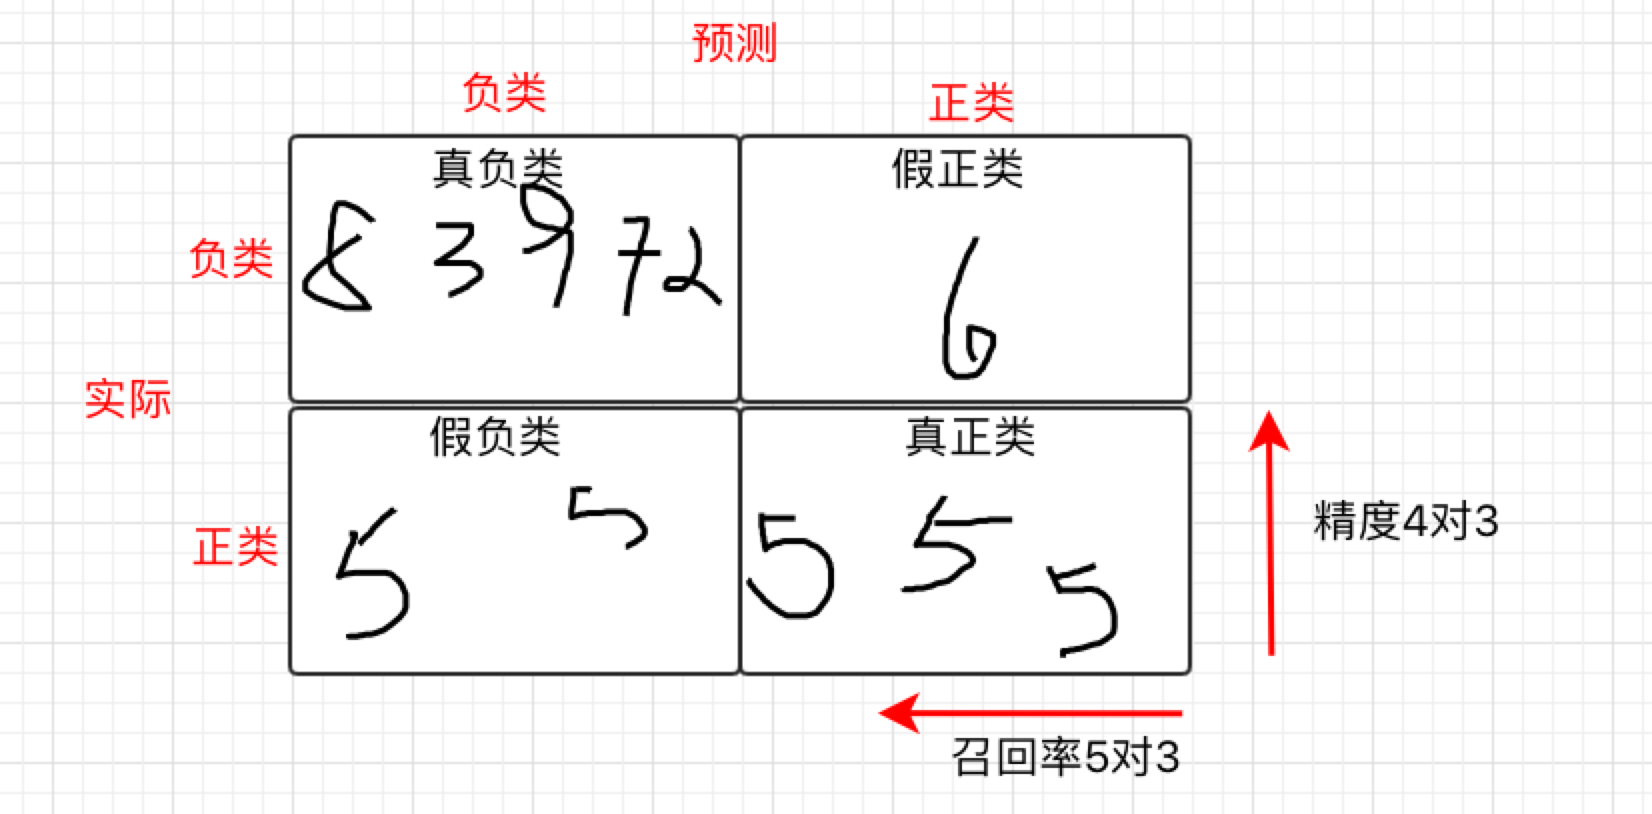
\includegraphics{./zhaohui.jpg}
\end{itemize}

    \hypertarget{ux7cbeux5ea6ux548cux53ecux56deux7387}{%
\subsection{精度和召回率}\label{ux7cbeux5ea6ux548cux53ecux56deux7387}}

    \begin{tcolorbox}[breakable, size=fbox, boxrule=1pt, pad at break*=1mm,colback=cellbackground, colframe=cellborder]
\prompt{In}{incolor}{23}{\boxspacing}
\begin{Verbatim}[commandchars=\\\{\}]
\PY{k+kn}{from} \PY{n+nn}{sklearn}\PY{n+nn}{.}\PY{n+nn}{metrics} \PY{k+kn}{import} \PY{n}{precision\PYZus{}score}\PY{p}{,} \PY{n}{recall\PYZus{}score}

\PY{n}{precision\PYZus{}score}\PY{p}{(}\PY{n}{y\PYZus{}train\PYZus{}5}\PY{p}{,} \PY{n}{y\PYZus{}train\PYZus{}pred}\PY{p}{)}  \PY{c+c1}{\PYZsh{} 精度 =  4327 / 4327 + 1276}
\end{Verbatim}
\end{tcolorbox}

            \begin{tcolorbox}[breakable, size=fbox, boxrule=.5pt, pad at break*=1mm, opacityfill=0]
\prompt{Out}{outcolor}{23}{\boxspacing}
\begin{Verbatim}[commandchars=\\\{\}]
0.8302614659237034
\end{Verbatim}
\end{tcolorbox}
        
    \begin{tcolorbox}[breakable, size=fbox, boxrule=1pt, pad at break*=1mm,colback=cellbackground, colframe=cellborder]
\prompt{In}{incolor}{24}{\boxspacing}
\begin{Verbatim}[commandchars=\\\{\}]
\PY{n}{recall\PYZus{}score}\PY{p}{(}\PY{n}{y\PYZus{}train\PYZus{}5}\PY{p}{,} \PY{n}{y\PYZus{}train\PYZus{}pred}\PY{p}{)}  \PY{c+c1}{\PYZsh{}  召回率 =  4327 / 4327 + 1094}
\end{Verbatim}
\end{tcolorbox}

            \begin{tcolorbox}[breakable, size=fbox, boxrule=.5pt, pad at break*=1mm, opacityfill=0]
\prompt{Out}{outcolor}{24}{\boxspacing}
\begin{Verbatim}[commandchars=\\\{\}]
0.7146282973621103
\end{Verbatim}
\end{tcolorbox}
        
    \begin{tcolorbox}[breakable, size=fbox, boxrule=1pt, pad at break*=1mm,colback=cellbackground, colframe=cellborder]
\prompt{In}{incolor}{25}{\boxspacing}
\begin{Verbatim}[commandchars=\\\{\}]
\PY{c+c1}{\PYZsh{} 说明 检测一张图的时候,只有90\PYZpc{}的概率是准确的,而且只有64\PYZpc{}的数字5 被它检测出来}
\PY{c+c1}{\PYZsh{} 精度和召回率合成单一指标,成为 F1 分数,谐波平均值}
\PY{c+c1}{\PYZsh{} 平均值平等对待所有的值,谐波平均值会给予较低值更高的权重,只有召回率和精度都很高时,才能获得较高的F1分数}
\end{Verbatim}
\end{tcolorbox}

    \begin{figure}
\centering
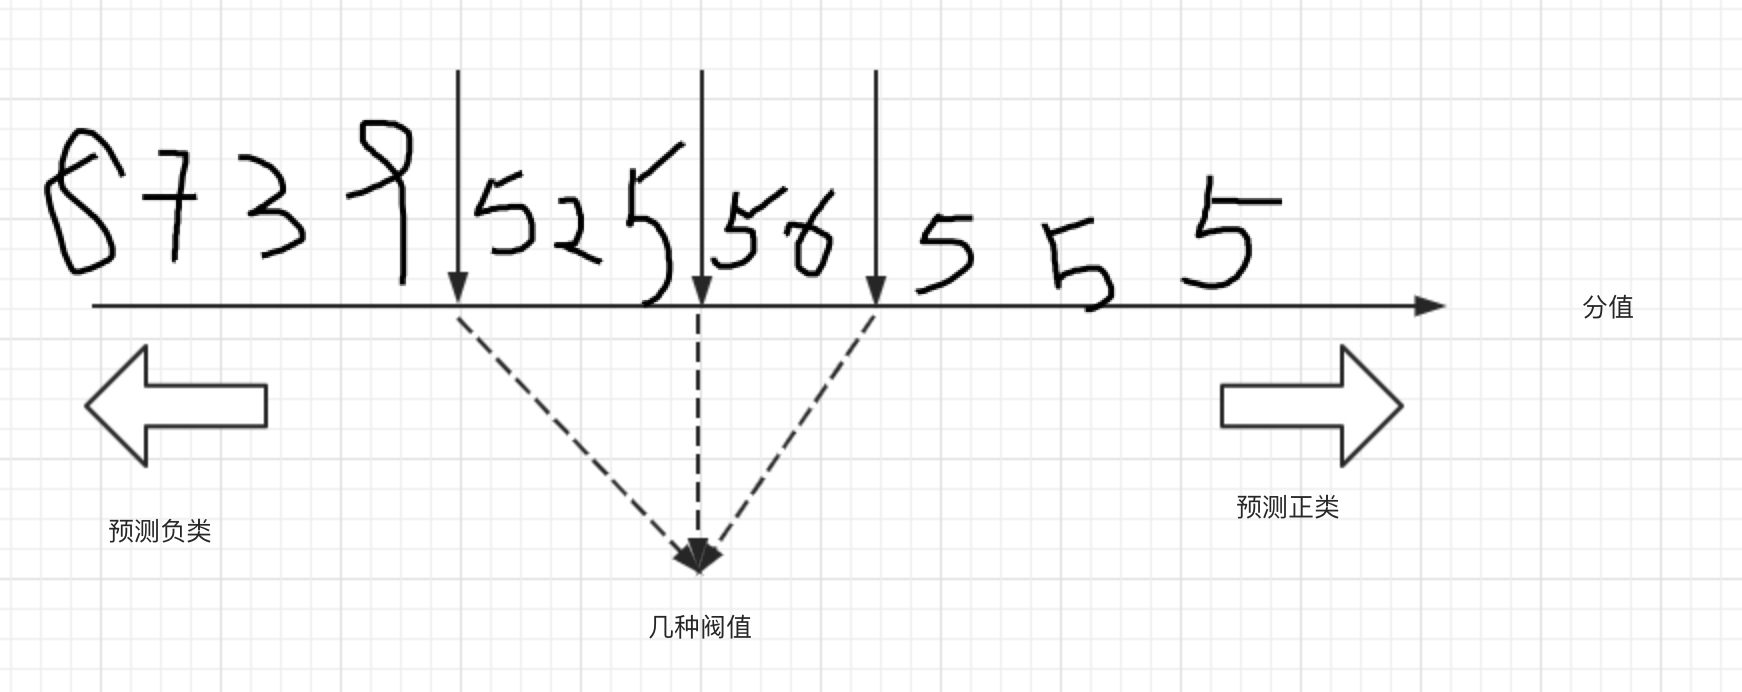
\includegraphics{./quanheng.jpg}
\caption{jupyter}
\end{figure}

    \begin{itemize}
\tightlist
\item
  SGDClassifier对每个实例基于决策函数计算一个分值,大于阀值为正类,否则为负类
\item
  中间阀值右侧找到4个真正类 真5 , 一个假正类 6, 精度为 4/5 80\%
\item
  在所有的6个 真正的5 中,分类器找到了4个,召回率为 4/6 67\%
\item
  提高阀值,向右移动,精度提高,召回降低
\item
  反之阀值降低,召回提高,精度降低
\item
  SKlearn不可以直接设置阀值,可以访问决策分数,
\item
  SGDClassifier 默认阀值为0
\end{itemize}

    \begin{tcolorbox}[breakable, size=fbox, boxrule=1pt, pad at break*=1mm,colback=cellbackground, colframe=cellborder]
\prompt{In}{incolor}{26}{\boxspacing}
\begin{Verbatim}[commandchars=\\\{\}]
\PY{c+c1}{\PYZsh{} 如何设置阀值}

\PY{c+c1}{\PYZsh{} 用predict\PYZus{}proba得到每个实例属于正类的概率,然后对概率切一下。以LogisticRegression为例}
\PY{c+c1}{\PYZsh{} clf = LogisticRegression()}
\PY{c+c1}{\PYZsh{} clf.fit(X\PYZus{}train, y\PYZus{}train)}
\PY{c+c1}{\PYZsh{} pred\PYZus{}proba = clf.predict\PYZus{}proba(X\PYZus{}test)[:, 1]}
\PY{c+c1}{\PYZsh{} threshold = 0.75  \PYZsh{} 阀值设置为0.75}
\PY{c+c1}{\PYZsh{} pred\PYZus{}label = pred\PYZus{}proba \PYZgt{} threshold}

\PY{c+c1}{\PYZsh{} pred\PYZus{}proba是每个实例为真的概率}
\PY{c+c1}{\PYZsh{} 假设阈值是0.75}
\PY{c+c1}{\PYZsh{} pred\PYZus{}label里True就是概率大于0.75的}
\end{Verbatim}
\end{tcolorbox}

    \begin{tcolorbox}[breakable, size=fbox, boxrule=1pt, pad at break*=1mm,colback=cellbackground, colframe=cellborder]
\prompt{In}{incolor}{27}{\boxspacing}
\begin{Verbatim}[commandchars=\\\{\}]
\PY{c+c1}{\PYZsh{} decision\PYZus{}function返回决策值}
\PY{n}{y\PYZus{}scores} \PY{o}{=} \PY{n}{sgd\PYZus{}clf}\PY{o}{.}\PY{n}{decision\PYZus{}function}\PY{p}{(}\PY{p}{[}\PY{n}{some\PYZus{}digit}\PY{p}{]}\PY{p}{)}
\PY{n}{y\PYZus{}scores}
\end{Verbatim}
\end{tcolorbox}

            \begin{tcolorbox}[breakable, size=fbox, boxrule=.5pt, pad at break*=1mm, opacityfill=0]
\prompt{Out}{outcolor}{27}{\boxspacing}
\begin{Verbatim}[commandchars=\\\{\}]
array([110731.97142777])
\end{Verbatim}
\end{tcolorbox}
        
    \begin{tcolorbox}[breakable, size=fbox, boxrule=1pt, pad at break*=1mm,colback=cellbackground, colframe=cellborder]
\prompt{In}{incolor}{28}{\boxspacing}
\begin{Verbatim}[commandchars=\\\{\}]
\PY{n}{threshold} \PY{o}{=} \PY{l+m+mi}{0}  \PY{c+c1}{\PYZsh{} 取阀值为0}
\PY{n}{y\PYZus{}some\PYZus{}digit\PYZus{}pred} \PY{o}{=} \PY{p}{(}\PY{n}{y\PYZus{}scores} \PY{o}{\PYZgt{}} \PY{n}{threshold}\PY{p}{)}  \PY{c+c1}{\PYZsh{} 判断决策值大于阀值}
\PY{n}{y\PYZus{}some\PYZus{}digit\PYZus{}pred}
\end{Verbatim}
\end{tcolorbox}

            \begin{tcolorbox}[breakable, size=fbox, boxrule=.5pt, pad at break*=1mm, opacityfill=0]
\prompt{Out}{outcolor}{28}{\boxspacing}
\begin{Verbatim}[commandchars=\\\{\}]
array([ True])
\end{Verbatim}
\end{tcolorbox}
        
    \begin{tcolorbox}[breakable, size=fbox, boxrule=1pt, pad at break*=1mm,colback=cellbackground, colframe=cellborder]
\prompt{In}{incolor}{29}{\boxspacing}
\begin{Verbatim}[commandchars=\\\{\}]
\PY{c+c1}{\PYZsh{} 提高阀值可以降低召回率,提高阀值到200000,就错了这个图}
\PY{n}{threshold} \PY{o}{=} \PY{l+m+mi}{200000}
\PY{n}{y\PYZus{}some\PYZus{}digit\PYZus{}pred} \PY{o}{=} \PY{p}{(}\PY{n}{y\PYZus{}scores} \PY{o}{\PYZgt{}} \PY{n}{threshold}\PY{p}{)}
\PY{n}{y\PYZus{}some\PYZus{}digit\PYZus{}pred}
\end{Verbatim}
\end{tcolorbox}

            \begin{tcolorbox}[breakable, size=fbox, boxrule=.5pt, pad at break*=1mm, opacityfill=0]
\prompt{Out}{outcolor}{29}{\boxspacing}
\begin{Verbatim}[commandchars=\\\{\}]
array([False])
\end{Verbatim}
\end{tcolorbox}
        
    \begin{tcolorbox}[breakable, size=fbox, boxrule=1pt, pad at break*=1mm,colback=cellbackground, colframe=cellborder]
\prompt{In}{incolor}{30}{\boxspacing}
\begin{Verbatim}[commandchars=\\\{\}]
\PY{c+c1}{\PYZsh{} 如何决定使用什么阀值}
\PY{c+c1}{\PYZsh{} 交叉预测decision\PYZus{}function返回决策值,而不是预测结果}
\PY{n}{y\PYZus{}scores} \PY{o}{=} \PY{n}{cross\PYZus{}val\PYZus{}predict}\PY{p}{(}\PY{n}{sgd\PYZus{}clf}\PY{p}{,} \PY{n}{X\PYZus{}train}\PY{p}{,} \PY{n}{y\PYZus{}train\PYZus{}5}\PY{p}{,} \PY{n}{cv}\PY{o}{=}\PY{l+m+mi}{3}\PY{p}{,}
                             \PY{n}{method}\PY{o}{=}\PY{l+s+s2}{\PYZdq{}}\PY{l+s+s2}{decision\PYZus{}function}\PY{l+s+s2}{\PYZdq{}}\PY{p}{)}
\end{Verbatim}
\end{tcolorbox}

    \begin{Verbatim}[commandchars=\\\{\}]
d:\textbackslash{}python3.7.5\textbackslash{}lib\textbackslash{}site-
packages\textbackslash{}sklearn\textbackslash{}linear\_model\textbackslash{}stochastic\_gradient.py:128: FutureWarning:
max\_iter and tol parameters have been added in <class
'sklearn.linear\_model.stochastic\_gradient.SGDClassifier'> in 0.19. If both are
left unset, they default to max\_iter=5 and tol=None. If tol is not None,
max\_iter defaults to max\_iter=1000. From 0.21, default max\_iter will be 1000,
and default tol will be 1e-3.
  "and default tol will be 1e-3." \% type(self), FutureWarning)
d:\textbackslash{}python3.7.5\textbackslash{}lib\textbackslash{}site-
packages\textbackslash{}sklearn\textbackslash{}linear\_model\textbackslash{}stochastic\_gradient.py:128: FutureWarning:
max\_iter and tol parameters have been added in <class
'sklearn.linear\_model.stochastic\_gradient.SGDClassifier'> in 0.19. If both are
left unset, they default to max\_iter=5 and tol=None. If tol is not None,
max\_iter defaults to max\_iter=1000. From 0.21, default max\_iter will be 1000,
and default tol will be 1e-3.
  "and default tol will be 1e-3." \% type(self), FutureWarning)
d:\textbackslash{}python3.7.5\textbackslash{}lib\textbackslash{}site-
packages\textbackslash{}sklearn\textbackslash{}linear\_model\textbackslash{}stochastic\_gradient.py:128: FutureWarning:
max\_iter and tol parameters have been added in <class
'sklearn.linear\_model.stochastic\_gradient.SGDClassifier'> in 0.19. If both are
left unset, they default to max\_iter=5 and tol=None. If tol is not None,
max\_iter defaults to max\_iter=1000. From 0.21, default max\_iter will be 1000,
and default tol will be 1e-3.
  "and default tol will be 1e-3." \% type(self), FutureWarning)
    \end{Verbatim}

    \begin{tcolorbox}[breakable, size=fbox, boxrule=1pt, pad at break*=1mm,colback=cellbackground, colframe=cellborder]
\prompt{In}{incolor}{31}{\boxspacing}
\begin{Verbatim}[commandchars=\\\{\}]
\PY{c+c1}{\PYZsh{} 有了y\PYZus{}scores,可以计算所有可能的阀值的精度和召回率}
\PY{n}{y\PYZus{}scores}\PY{o}{.}\PY{n}{shape}
\end{Verbatim}
\end{tcolorbox}

            \begin{tcolorbox}[breakable, size=fbox, boxrule=.5pt, pad at break*=1mm, opacityfill=0]
\prompt{Out}{outcolor}{31}{\boxspacing}
\begin{Verbatim}[commandchars=\\\{\}]
(60000,)
\end{Verbatim}
\end{tcolorbox}
        
    \hypertarget{prprecision---recallux66f2ux7ebf}{%
\subsection{PR(Precision -
Recall)曲线}\label{prprecision---recallux66f2ux7ebf}}

\textbf{正类非常少或者更关注假正类而不是假负类} - 绘制精度和召回率

    \begin{enumerate}
\def\labelenumi{\arabic{enumi}.}
\tightlist
\item
  绘制精度和召回相对于阀值的函数图
\end{enumerate}

    \begin{tcolorbox}[breakable, size=fbox, boxrule=1pt, pad at break*=1mm,colback=cellbackground, colframe=cellborder]
\prompt{In}{incolor}{32}{\boxspacing}
\begin{Verbatim}[commandchars=\\\{\}]
\PY{k+kn}{from} \PY{n+nn}{sklearn}\PY{n+nn}{.}\PY{n+nn}{metrics} \PY{k+kn}{import} \PY{n}{precision\PYZus{}recall\PYZus{}curve}

\PY{c+c1}{\PYZsh{} 传入是5标签y\PYZus{}train\PYZus{}5和决策值数组y\PYZus{}scores  取得精度 召回率 阀值}
\PY{n}{precisions}\PY{p}{,} \PY{n}{recalls}\PY{p}{,} \PY{n}{thresholds} \PY{o}{=} \PY{n}{precision\PYZus{}recall\PYZus{}curve}\PY{p}{(}\PY{n}{y\PYZus{}train\PYZus{}5}\PY{p}{,} \PY{n}{y\PYZus{}scores}\PY{p}{)}
\end{Verbatim}
\end{tcolorbox}

    \begin{tcolorbox}[breakable, size=fbox, boxrule=1pt, pad at break*=1mm,colback=cellbackground, colframe=cellborder]
\prompt{In}{incolor}{33}{\boxspacing}
\begin{Verbatim}[commandchars=\\\{\}]
\PY{c+c1}{\PYZsh{} 使用matplotlib 绘制精度和召回相对于阀值的函数图}
\PY{k}{def} \PY{n+nf}{plot\PYZus{}precision\PYZus{}recall\PYZus{}vs\PYZus{}threshold}\PY{p}{(}\PY{n}{precisions}\PY{p}{,} \PY{n}{recalls}\PY{p}{,} \PY{n}{thresholds}\PY{p}{)}\PY{p}{:}
    \PY{c+c1}{\PYZsh{} 以阀值为横轴x 以精度为纵轴y 绘制曲线}
    \PY{n}{plt}\PY{o}{.}\PY{n}{plot}\PY{p}{(}\PY{n}{thresholds}\PY{p}{,} \PY{n}{precisions}\PY{p}{[}\PY{p}{:}\PY{o}{\PYZhy{}}\PY{l+m+mi}{1}\PY{p}{]}\PY{p}{,} \PY{l+s+s2}{\PYZdq{}}\PY{l+s+s2}{b\PYZhy{}\PYZhy{}}\PY{l+s+s2}{\PYZdq{}}\PY{p}{,} \PY{n}{label}\PY{o}{=}\PY{l+s+s2}{\PYZdq{}}\PY{l+s+s2}{Precision}\PY{l+s+s2}{\PYZdq{}}\PY{p}{,} \PY{n}{linewidth}\PY{o}{=}\PY{l+m+mi}{2}\PY{p}{)}
    \PY{c+c1}{\PYZsh{} 以阀值为横轴x 以召回为纵轴y 绘制曲线}
    \PY{n}{plt}\PY{o}{.}\PY{n}{plot}\PY{p}{(}\PY{n}{thresholds}\PY{p}{,} \PY{n}{recalls}\PY{p}{[}\PY{p}{:}\PY{o}{\PYZhy{}}\PY{l+m+mi}{1}\PY{p}{]}\PY{p}{,} \PY{l+s+s2}{\PYZdq{}}\PY{l+s+s2}{g\PYZhy{}}\PY{l+s+s2}{\PYZdq{}}\PY{p}{,} \PY{n}{label}\PY{o}{=}\PY{l+s+s2}{\PYZdq{}}\PY{l+s+s2}{Recall}\PY{l+s+s2}{\PYZdq{}}\PY{p}{,} \PY{n}{linewidth}\PY{o}{=}\PY{l+m+mi}{2}\PY{p}{)}
    \PY{c+c1}{\PYZsh{} 横轴文本框}
    \PY{n}{plt}\PY{o}{.}\PY{n}{xlabel}\PY{p}{(}\PY{l+s+s2}{\PYZdq{}}\PY{l+s+s2}{Threshold}\PY{l+s+s2}{\PYZdq{}}\PY{p}{,} \PY{n}{fontsize}\PY{o}{=}\PY{l+m+mi}{16}\PY{p}{)}
    \PY{c+c1}{\PYZsh{} 显示提示框}
    \PY{n}{plt}\PY{o}{.}\PY{n}{legend}\PY{p}{(}\PY{n}{loc}\PY{o}{=}\PY{l+s+s2}{\PYZdq{}}\PY{l+s+s2}{upper left}\PY{l+s+s2}{\PYZdq{}}\PY{p}{,} \PY{n}{fontsize}\PY{o}{=}\PY{l+m+mi}{16}\PY{p}{)}
    \PY{c+c1}{\PYZsh{} 纵轴限制起始0至1}
    \PY{n}{plt}\PY{o}{.}\PY{n}{ylim}\PY{p}{(}\PY{p}{[}\PY{l+m+mi}{0}\PY{p}{,} \PY{l+m+mi}{1}\PY{p}{]}\PY{p}{)}

\PY{c+c1}{\PYZsh{} 配置图片大小}
\PY{n}{plt}\PY{o}{.}\PY{n}{figure}\PY{p}{(}\PY{n}{figsize}\PY{o}{=}\PY{p}{(}\PY{l+m+mi}{8}\PY{p}{,} \PY{l+m+mi}{4}\PY{p}{)}\PY{p}{)}
\PY{c+c1}{\PYZsh{} 调用函数传入参数,绘制出曲线}
\PY{n}{plot\PYZus{}precision\PYZus{}recall\PYZus{}vs\PYZus{}threshold}\PY{p}{(}\PY{n}{precisions}\PY{p}{,} \PY{n}{recalls}\PY{p}{,} \PY{n}{thresholds}\PY{p}{)}
\PY{c+c1}{\PYZsh{} 横轴限制起始}
\PY{n}{plt}\PY{o}{.}\PY{n}{xlim}\PY{p}{(}\PY{p}{[}\PY{o}{\PYZhy{}}\PY{l+m+mi}{700000}\PY{p}{,} \PY{l+m+mi}{700000}\PY{p}{]}\PY{p}{)}
\PY{c+c1}{\PYZsh{} 显示图片}
\PY{n}{plt}\PY{o}{.}\PY{n}{show}\PY{p}{(}\PY{p}{)}
\end{Verbatim}
\end{tcolorbox}

    \begin{center}
    \adjustimage{max size={0.9\linewidth}{0.9\paperheight}}{MNIST_Classify_files/MNIST_Classify_50_0.png}
    \end{center}
    { \hspace*{\fill} \\}
    
    \begin{enumerate}
\def\labelenumi{\arabic{enumi}.}
\setcounter{enumi}{1}
\tightlist
\item
  精度和召回的曲线图
\end{enumerate}

    \begin{tcolorbox}[breakable, size=fbox, boxrule=1pt, pad at break*=1mm,colback=cellbackground, colframe=cellborder]
\prompt{In}{incolor}{34}{\boxspacing}
\begin{Verbatim}[commandchars=\\\{\}]
\PY{n}{plt}\PY{o}{.}\PY{n}{rcParams}\PY{p}{[}\PY{l+s+s1}{\PYZsq{}}\PY{l+s+s1}{font.sans\PYZhy{}serif}\PY{l+s+s1}{\PYZsq{}}\PY{p}{]} \PY{o}{=} \PY{p}{[}\PY{l+s+s1}{\PYZsq{}}\PY{l+s+s1}{SimHei}\PY{l+s+s1}{\PYZsq{}}\PY{p}{]}

\PY{c+c1}{\PYZsh{} 以召回为横轴x 以精度为纵轴y 绘制曲线}
\PY{k}{def} \PY{n+nf}{plot\PYZus{}precision\PYZus{}vs\PYZus{}recall}\PY{p}{(}\PY{n}{precisions}\PY{p}{,} \PY{n}{recalls}\PY{p}{)}\PY{p}{:}
    \PY{c+c1}{\PYZsh{} 以召回为横轴x 以精度为纵轴y 绘制曲线}
    \PY{n}{plt}\PY{o}{.}\PY{n}{plot}\PY{p}{(}\PY{n}{recalls}\PY{p}{,} \PY{n}{precisions}\PY{p}{,} \PY{l+s+s2}{\PYZdq{}}\PY{l+s+s2}{b\PYZhy{}}\PY{l+s+s2}{\PYZdq{}}\PY{p}{,} \PY{n}{linewidth}\PY{o}{=}\PY{l+m+mi}{2}\PY{p}{)}
    \PY{c+c1}{\PYZsh{} 横轴文本框}
    \PY{n}{plt}\PY{o}{.}\PY{n}{xlabel}\PY{p}{(}\PY{l+s+s2}{\PYZdq{}}\PY{l+s+s2}{召回}\PY{l+s+s2}{\PYZdq{}}\PY{p}{,} \PY{n}{fontsize}\PY{o}{=}\PY{l+m+mi}{16}\PY{p}{)}
    \PY{c+c1}{\PYZsh{} 纵轴文本框}
    \PY{n}{plt}\PY{o}{.}\PY{n}{ylabel}\PY{p}{(}\PY{l+s+s2}{\PYZdq{}}\PY{l+s+s2}{精度}\PY{l+s+s2}{\PYZdq{}}\PY{p}{,} \PY{n}{fontsize}\PY{o}{=}\PY{l+m+mi}{16}\PY{p}{)}
    \PY{n}{plt}\PY{o}{.}\PY{n}{axis}\PY{p}{(}\PY{p}{[}\PY{l+m+mi}{0}\PY{p}{,} \PY{l+m+mi}{1}\PY{p}{,} \PY{l+m+mi}{0}\PY{p}{,} \PY{l+m+mi}{1}\PY{p}{]}\PY{p}{)}

\PY{n}{plt}\PY{o}{.}\PY{n}{figure}\PY{p}{(}\PY{n}{figsize}\PY{o}{=}\PY{p}{(}\PY{l+m+mi}{8}\PY{p}{,} \PY{l+m+mi}{6}\PY{p}{)}\PY{p}{)}
\PY{n}{plot\PYZus{}precision\PYZus{}vs\PYZus{}recall}\PY{p}{(}\PY{n}{precisions}\PY{p}{,} \PY{n}{recalls}\PY{p}{)}
\PY{n}{plt}\PY{o}{.}\PY{n}{show}\PY{p}{(}\PY{p}{)}
\end{Verbatim}
\end{tcolorbox}

    \begin{center}
    \adjustimage{max size={0.9\linewidth}{0.9\paperheight}}{MNIST_Classify_files/MNIST_Classify_52_0.png}
    \end{center}
    { \hspace*{\fill} \\}
    
    \hypertarget{ux901aux8fc7ux9009ux62e9ux9600ux503cux6765ux5b9eux73b0ux6700ux4f73ux7684ux7cbeux5ea6ux53ecux56deux7387ux6743ux8861}{%
\subsection{通过选择阀值来实现最佳的精度/召回率权衡}\label{ux901aux8fc7ux9009ux62e9ux9600ux503cux6765ux5b9eux73b0ux6700ux4f73ux7684ux7cbeux5ea6ux53ecux56deux7387ux6743ux8861}}

    \begin{tcolorbox}[breakable, size=fbox, boxrule=1pt, pad at break*=1mm,colback=cellbackground, colframe=cellborder]
\prompt{In}{incolor}{35}{\boxspacing}
\begin{Verbatim}[commandchars=\\\{\}]
\PY{c+c1}{\PYZsh{} 目标设定为90\PYZpc{}的精度,阀值大概在30000左右 , 设置了阀值为30000}
\PY{n}{y\PYZus{}train\PYZus{}pred\PYZus{}90} \PY{o}{=} \PY{p}{(}\PY{n}{y\PYZus{}scores} \PY{o}{\PYZgt{}} \PY{l+m+mi}{30000}\PY{p}{)}
\end{Verbatim}
\end{tcolorbox}

    \begin{tcolorbox}[breakable, size=fbox, boxrule=1pt, pad at break*=1mm,colback=cellbackground, colframe=cellborder]
\prompt{In}{incolor}{36}{\boxspacing}
\begin{Verbatim}[commandchars=\\\{\}]
\PY{n}{precision\PYZus{}score}\PY{p}{(}\PY{n}{y\PYZus{}train\PYZus{}5}\PY{p}{,} \PY{n}{y\PYZus{}train\PYZus{}pred\PYZus{}90}\PY{p}{)}
\end{Verbatim}
\end{tcolorbox}

            \begin{tcolorbox}[breakable, size=fbox, boxrule=.5pt, pad at break*=1mm, opacityfill=0]
\prompt{Out}{outcolor}{36}{\boxspacing}
\begin{Verbatim}[commandchars=\\\{\}]
0.8626701695724862
\end{Verbatim}
\end{tcolorbox}
        
    \begin{tcolorbox}[breakable, size=fbox, boxrule=1pt, pad at break*=1mm,colback=cellbackground, colframe=cellborder]
\prompt{In}{incolor}{37}{\boxspacing}
\begin{Verbatim}[commandchars=\\\{\}]
\PY{n}{recall\PYZus{}score}\PY{p}{(}\PY{n}{y\PYZus{}train\PYZus{}5}\PY{p}{,} \PY{n}{y\PYZus{}train\PYZus{}pred\PYZus{}90}\PY{p}{)}
\end{Verbatim}
\end{tcolorbox}

            \begin{tcolorbox}[breakable, size=fbox, boxrule=.5pt, pad at break*=1mm, opacityfill=0]
\prompt{Out}{outcolor}{37}{\boxspacing}
\begin{Verbatim}[commandchars=\\\{\}]
0.6662977310459325
\end{Verbatim}
\end{tcolorbox}
        
    \hypertarget{ux7cbeux5ea6ux53ecux56deux603bux7ed3}{%
\subsection{精度召回总结}\label{ux7cbeux5ea6ux53ecux56deux603bux7ed3}}

\begin{itemize}
\tightlist
\item
  获得了一个90\%精度的分类器,但如果召回太低,精度再高,也不怎么有用
\item
  如果工作中,需要\textbf{99\%的精度},你应该回应,\textbf{召回率}是多少?
\end{itemize}

    \hypertarget{roc-ux66f2ux7ebf}{%
\subsection{ROC 曲线}\label{roc-ux66f2ux7ebf}}

Receiver Operating Characteristic
Curve,中文名字叫``受试者工作特征曲线'' - 本质是
\textbf{真正类率TPR}和\textbf{假正类率FPR}\_\_的比例\_\_(错误的分为正类的负类实例比例)
- 与召回/精度曲线非常相似

    \begin{tcolorbox}[breakable, size=fbox, boxrule=1pt, pad at break*=1mm,colback=cellbackground, colframe=cellborder]
\prompt{In}{incolor}{38}{\boxspacing}
\begin{Verbatim}[commandchars=\\\{\}]
\PY{k+kn}{from} \PY{n+nn}{sklearn}\PY{n+nn}{.}\PY{n+nn}{metrics} \PY{k+kn}{import} \PY{n}{roc\PYZus{}curve}

\PY{n}{fpr}\PY{p}{,} \PY{n}{tpr}\PY{p}{,} \PY{n}{thresholds} \PY{o}{=} \PY{n}{roc\PYZus{}curve}\PY{p}{(}\PY{n}{y\PYZus{}train\PYZus{}5}\PY{p}{,} \PY{n}{y\PYZus{}scores}\PY{p}{)}
\end{Verbatim}
\end{tcolorbox}

    \begin{tcolorbox}[breakable, size=fbox, boxrule=1pt, pad at break*=1mm,colback=cellbackground, colframe=cellborder]
\prompt{In}{incolor}{39}{\boxspacing}
\begin{Verbatim}[commandchars=\\\{\}]
\PY{n}{plt}\PY{o}{.}\PY{n}{rcParams}\PY{p}{[}\PY{l+s+s1}{\PYZsq{}}\PY{l+s+s1}{font.sans\PYZhy{}serif}\PY{l+s+s1}{\PYZsq{}}\PY{p}{]} \PY{o}{=} \PY{p}{[}\PY{l+s+s1}{\PYZsq{}}\PY{l+s+s1}{SimHei}\PY{l+s+s1}{\PYZsq{}}\PY{p}{]}
\PY{k}{def} \PY{n+nf}{plot\PYZus{}roc\PYZus{}curve}\PY{p}{(}\PY{n}{fpr}\PY{p}{,} \PY{n}{tpr}\PY{p}{,} \PY{n}{label}\PY{o}{=}\PY{k+kc}{None}\PY{p}{)}\PY{p}{:}
    \PY{n}{plt}\PY{o}{.}\PY{n}{plot}\PY{p}{(}\PY{n}{fpr}\PY{p}{,} \PY{n}{tpr}\PY{p}{,} \PY{n}{linewidth}\PY{o}{=}\PY{l+m+mi}{2}\PY{p}{,} \PY{n}{label}\PY{o}{=}\PY{n}{label}\PY{p}{)}
    \PY{n}{plt}\PY{o}{.}\PY{n}{plot}\PY{p}{(}\PY{p}{[}\PY{l+m+mi}{0}\PY{p}{,} \PY{l+m+mi}{1}\PY{p}{]}\PY{p}{,} \PY{p}{[}\PY{l+m+mi}{0}\PY{p}{,} \PY{l+m+mi}{1}\PY{p}{]}\PY{p}{,} \PY{l+s+s1}{\PYZsq{}}\PY{l+s+s1}{k\PYZhy{}\PYZhy{}}\PY{l+s+s1}{\PYZsq{}}\PY{p}{)}
    \PY{n}{plt}\PY{o}{.}\PY{n}{axis}\PY{p}{(}\PY{p}{[}\PY{l+m+mi}{0}\PY{p}{,} \PY{l+m+mi}{1}\PY{p}{,} \PY{l+m+mi}{0}\PY{p}{,} \PY{l+m+mi}{1}\PY{p}{]}\PY{p}{)}
    \PY{n}{plt}\PY{o}{.}\PY{n}{xlabel}\PY{p}{(}\PY{l+s+s1}{\PYZsq{}}\PY{l+s+s1}{假正类率}\PY{l+s+s1}{\PYZsq{}}\PY{p}{,} \PY{n}{fontsize}\PY{o}{=}\PY{l+m+mi}{16}\PY{p}{)}
    \PY{n}{plt}\PY{o}{.}\PY{n}{ylabel}\PY{p}{(}\PY{l+s+s1}{\PYZsq{}}\PY{l+s+s1}{真正类率}\PY{l+s+s1}{\PYZsq{}}\PY{p}{,} \PY{n}{fontsize}\PY{o}{=}\PY{l+m+mi}{16}\PY{p}{)}

\PY{n}{plt}\PY{o}{.}\PY{n}{figure}\PY{p}{(}\PY{n}{figsize}\PY{o}{=}\PY{p}{(}\PY{l+m+mi}{8}\PY{p}{,} \PY{l+m+mi}{6}\PY{p}{)}\PY{p}{)}
\PY{n}{plot\PYZus{}roc\PYZus{}curve}\PY{p}{(}\PY{n}{fpr}\PY{p}{,} \PY{n}{tpr}\PY{p}{)}

\PY{n}{plt}\PY{o}{.}\PY{n}{show}\PY{p}{(}\PY{p}{)}
\end{Verbatim}
\end{tcolorbox}

    \begin{center}
    \adjustimage{max size={0.9\linewidth}{0.9\paperheight}}{MNIST_Classify_files/MNIST_Classify_60_0.png}
    \end{center}
    { \hspace*{\fill} \\}
    
    \hypertarget{aucarea-under-curve}{%
\subsubsection{AUC(Area Under Curve)}\label{aucarea-under-curve}}

\begin{itemize}
\tightlist
\item
  被定义为ROC曲线下与坐标轴围成的面积,显然这个面积的数值不会大于1
\end{itemize}

    \begin{tcolorbox}[breakable, size=fbox, boxrule=1pt, pad at break*=1mm,colback=cellbackground, colframe=cellborder]
\prompt{In}{incolor}{40}{\boxspacing}
\begin{Verbatim}[commandchars=\\\{\}]
\PY{c+c1}{\PYZsh{} 计算曲线下面积AUC,虚线是随机分类0.5到1}
\PY{k+kn}{from} \PY{n+nn}{sklearn}\PY{n+nn}{.}\PY{n+nn}{metrics} \PY{k+kn}{import} \PY{n}{roc\PYZus{}auc\PYZus{}score}

\PY{n}{roc\PYZus{}auc\PYZus{}score}\PY{p}{(}\PY{n}{y\PYZus{}train\PYZus{}5}\PY{p}{,} \PY{n}{y\PYZus{}scores}\PY{p}{)}
\end{Verbatim}
\end{tcolorbox}

            \begin{tcolorbox}[breakable, size=fbox, boxrule=.5pt, pad at break*=1mm, opacityfill=0]
\prompt{Out}{outcolor}{40}{\boxspacing}
\begin{Verbatim}[commandchars=\\\{\}]
0.9586344817908701
\end{Verbatim}
\end{tcolorbox}
        
    \hypertarget{prux548crocux603bux7ed3}{%
\subsection{PR和ROC总结}\label{prux548crocux603bux7ed3}}

\begin{itemize}
\tightlist
\item
  关于PR曲线:召回率越高,分类器的假正类率FPR就越高
\item
  ROC的虚线表示纯随机分类器的曲线,好的分类器应该远离这条线,向左上角靠拢
\item
  是使用精度/召回率 PR曲线,还是使用ROC,关键在于
  正类非常少或者更关注假正类而不是假负类,选择PR,反之ROC
\item
  例如:前面例子PR曲线很不错是因为跟负类 非5 相比, 正类 数据5
  数量真的很少
\end{itemize}

    \hypertarget{ux8badux7ec3ux968fux673aux68eeux6797ux5206ux7c7bux5668ux6bd4ux8f83sgdux5206ux7c7bux5668ux7684rocux66f2ux7ebfux548croc-aucux5206ux6570}{%
\subsection{训练随机森林分类器,比较SGD分类器的ROC曲线和ROC
AUC分数}\label{ux8badux7ec3ux968fux673aux68eeux6797ux5206ux7c7bux5668ux6bd4ux8f83sgdux5206ux7c7bux5668ux7684rocux66f2ux7ebfux548croc-aucux5206ux6570}}

    \begin{itemize}
\tightlist
\item
  获取训练集中每个实例的分数
\item
  \textbf{RandomForestClassifier
  没有descision\_function(),但是拥有dict\_proda()方法,sklearn中分类器都有这两个中的一个}
\item
  dict\_proda\textbf{返回一个矩阵},每行一个实例,每列代表一个类别的概率,比如这个图片
  70\%是5
\end{itemize}

    \begin{tcolorbox}[breakable, size=fbox, boxrule=1pt, pad at break*=1mm,colback=cellbackground, colframe=cellborder]
\prompt{In}{incolor}{41}{\boxspacing}
\begin{Verbatim}[commandchars=\\\{\}]
\PY{k+kn}{from} \PY{n+nn}{sklearn}\PY{n+nn}{.}\PY{n+nn}{ensemble} \PY{k+kn}{import} \PY{n}{RandomForestClassifier}
\PY{n}{forest\PYZus{}clf} \PY{o}{=} \PY{n}{RandomForestClassifier}\PY{p}{(}\PY{n}{n\PYZus{}estimators}\PY{o}{=}\PY{l+m+mi}{10}\PY{p}{,} \PY{n}{random\PYZus{}state}\PY{o}{=}\PY{l+m+mi}{42}\PY{p}{)}
\PY{n}{y\PYZus{}probas\PYZus{}forest} \PY{o}{=} \PY{n}{cross\PYZus{}val\PYZus{}predict}\PY{p}{(}\PY{n}{forest\PYZus{}clf}\PY{p}{,} \PY{n}{X\PYZus{}train}\PY{p}{,} \PY{n}{y\PYZus{}train\PYZus{}5}\PY{p}{,} \PY{n}{cv}\PY{o}{=}\PY{l+m+mi}{3}\PY{p}{,}
                                    \PY{n}{method}\PY{o}{=}\PY{l+s+s2}{\PYZdq{}}\PY{l+s+s2}{predict\PYZus{}proba}\PY{l+s+s2}{\PYZdq{}}\PY{p}{)}
\end{Verbatim}
\end{tcolorbox}

    \begin{Verbatim}[commandchars=\\\{\}]
d:\textbackslash{}python3.7.5\textbackslash{}lib\textbackslash{}site-packages\textbackslash{}sklearn\textbackslash{}ensemble\textbackslash{}weight\_boosting.py:29:
DeprecationWarning: numpy.core.umath\_tests is an internal NumPy module and
should not be imported. It will be removed in a future NumPy release.
  from numpy.core.umath\_tests import inner1d
    \end{Verbatim}

    \begin{tcolorbox}[breakable, size=fbox, boxrule=1pt, pad at break*=1mm,colback=cellbackground, colframe=cellborder]
\prompt{In}{incolor}{42}{\boxspacing}
\begin{Verbatim}[commandchars=\\\{\}]
\PY{c+c1}{\PYZsh{} 两列,第一列为是的概率,第二列为不是的概率  每一行两列概率之和为1}
\PY{n}{y\PYZus{}probas\PYZus{}forest}  \PY{c+c1}{\PYZsh{} 矩阵内的数都是类别的概率}
\end{Verbatim}
\end{tcolorbox}

            \begin{tcolorbox}[breakable, size=fbox, boxrule=.5pt, pad at break*=1mm, opacityfill=0]
\prompt{Out}{outcolor}{42}{\boxspacing}
\begin{Verbatim}[commandchars=\\\{\}]
array([[1. , 0. ],
       [1. , 0. ],
       [1. , 0. ],
       {\ldots},
       [0.1, 0.9],
       [1. , 0. ],
       [1. , 0. ]])
\end{Verbatim}
\end{tcolorbox}
        
    \begin{tcolorbox}[breakable, size=fbox, boxrule=1pt, pad at break*=1mm,colback=cellbackground, colframe=cellborder]
\prompt{In}{incolor}{43}{\boxspacing}
\begin{Verbatim}[commandchars=\\\{\}]
\PY{c+c1}{\PYZsh{} 绘制ROC曲线,需要决策值不是概率}
\PY{c+c1}{\PYZsh{} 此处直接使用正类的概率作为决策值:}
\PY{n}{y\PYZus{}scores\PYZus{}forest} \PY{o}{=} \PY{n}{y\PYZus{}probas\PYZus{}forest}\PY{p}{[}\PY{p}{:}\PY{p}{,} \PY{l+m+mi}{1}\PY{p}{]}  \PY{c+c1}{\PYZsh{} 取概率为是的一列}

\PY{c+c1}{\PYZsh{} FPR TPR 阀值}
\PY{n}{fpr\PYZus{}forest}\PY{p}{,} \PY{n}{tpr\PYZus{}forest}\PY{p}{,} \PY{n}{thresholds\PYZus{}forest} \PY{o}{=} \PY{n}{roc\PYZus{}curve}\PY{p}{(}\PY{n}{y\PYZus{}train\PYZus{}5}\PY{p}{,}\PY{n}{y\PYZus{}scores\PYZus{}forest}\PY{p}{)}
\end{Verbatim}
\end{tcolorbox}

    \begin{tcolorbox}[breakable, size=fbox, boxrule=1pt, pad at break*=1mm,colback=cellbackground, colframe=cellborder]
\prompt{In}{incolor}{44}{\boxspacing}
\begin{Verbatim}[commandchars=\\\{\}]
\PY{n}{y\PYZus{}scores\PYZus{}forest}
\end{Verbatim}
\end{tcolorbox}

            \begin{tcolorbox}[breakable, size=fbox, boxrule=.5pt, pad at break*=1mm, opacityfill=0]
\prompt{Out}{outcolor}{44}{\boxspacing}
\begin{Verbatim}[commandchars=\\\{\}]
array([0. , 0. , 0. , {\ldots}, 0.9, 0. , 0. ])
\end{Verbatim}
\end{tcolorbox}
        
    \begin{tcolorbox}[breakable, size=fbox, boxrule=1pt, pad at break*=1mm,colback=cellbackground, colframe=cellborder]
\prompt{In}{incolor}{45}{\boxspacing}
\begin{Verbatim}[commandchars=\\\{\}]
\PY{n}{plt}\PY{o}{.}\PY{n}{figure}\PY{p}{(}\PY{n}{figsize}\PY{o}{=}\PY{p}{(}\PY{l+m+mi}{8}\PY{p}{,} \PY{l+m+mi}{6}\PY{p}{)}\PY{p}{)}
\PY{n}{plt}\PY{o}{.}\PY{n}{plot}\PY{p}{(}\PY{n}{fpr}\PY{p}{,} \PY{n}{tpr}\PY{p}{,} \PY{l+s+s2}{\PYZdq{}}\PY{l+s+s2}{b:}\PY{l+s+s2}{\PYZdq{}}\PY{p}{,} \PY{n}{linewidth}\PY{o}{=}\PY{l+m+mi}{2}\PY{p}{,} \PY{n}{label}\PY{o}{=}\PY{l+s+s2}{\PYZdq{}}\PY{l+s+s2}{SGD}\PY{l+s+s2}{\PYZdq{}}\PY{p}{)}
\PY{n}{plot\PYZus{}roc\PYZus{}curve}\PY{p}{(}\PY{n}{fpr\PYZus{}forest}\PY{p}{,} \PY{n}{tpr\PYZus{}forest}\PY{p}{,} \PY{l+s+s2}{\PYZdq{}}\PY{l+s+s2}{Random Forest}\PY{l+s+s2}{\PYZdq{}}\PY{p}{)}
\PY{n}{plt}\PY{o}{.}\PY{n}{legend}\PY{p}{(}\PY{n}{loc}\PY{o}{=}\PY{l+s+s2}{\PYZdq{}}\PY{l+s+s2}{lower right}\PY{l+s+s2}{\PYZdq{}}\PY{p}{,} \PY{n}{fontsize}\PY{o}{=}\PY{l+m+mi}{16}\PY{p}{)}
\PY{n}{plt}\PY{o}{.}\PY{n}{show}\PY{p}{(}\PY{p}{)}
\end{Verbatim}
\end{tcolorbox}

    \begin{center}
    \adjustimage{max size={0.9\linewidth}{0.9\paperheight}}{MNIST_Classify_files/MNIST_Classify_70_0.png}
    \end{center}
    { \hspace*{\fill} \\}
    
    \begin{tcolorbox}[breakable, size=fbox, boxrule=1pt, pad at break*=1mm,colback=cellbackground, colframe=cellborder]
\prompt{In}{incolor}{46}{\boxspacing}
\begin{Verbatim}[commandchars=\\\{\}]
\PY{c+c1}{\PYZsh{} Rand 比SGD 好很多,ROC AUC的分数也高很多}
\PY{n}{roc\PYZus{}auc\PYZus{}score}\PY{p}{(}\PY{n}{y\PYZus{}train\PYZus{}5}\PY{p}{,} \PY{n}{y\PYZus{}scores\PYZus{}forest}\PY{p}{)}
\end{Verbatim}
\end{tcolorbox}

            \begin{tcolorbox}[breakable, size=fbox, boxrule=.5pt, pad at break*=1mm, opacityfill=0]
\prompt{Out}{outcolor}{46}{\boxspacing}
\begin{Verbatim}[commandchars=\\\{\}]
0.9922621112273469
\end{Verbatim}
\end{tcolorbox}
        
    \begin{tcolorbox}[breakable, size=fbox, boxrule=1pt, pad at break*=1mm,colback=cellbackground, colframe=cellborder]
\prompt{In}{incolor}{47}{\boxspacing}
\begin{Verbatim}[commandchars=\\\{\}]
\PY{c+c1}{\PYZsh{} 再看一下 精度和召回率 也很高}
\PY{n}{y\PYZus{}train\PYZus{}pred\PYZus{}forest} \PY{o}{=} \PY{n}{cross\PYZus{}val\PYZus{}predict}\PY{p}{(}\PY{n}{forest\PYZus{}clf}\PY{p}{,} \PY{n}{X\PYZus{}train}\PY{p}{,} \PY{n}{y\PYZus{}train\PYZus{}5}\PY{p}{,} \PY{n}{cv}\PY{o}{=}\PY{l+m+mi}{3}\PY{p}{)}
\PY{n}{precision\PYZus{}score}\PY{p}{(}\PY{n}{y\PYZus{}train\PYZus{}5}\PY{p}{,} \PY{n}{y\PYZus{}train\PYZus{}pred\PYZus{}forest}\PY{p}{)}
\end{Verbatim}
\end{tcolorbox}

            \begin{tcolorbox}[breakable, size=fbox, boxrule=.5pt, pad at break*=1mm, opacityfill=0]
\prompt{Out}{outcolor}{47}{\boxspacing}
\begin{Verbatim}[commandchars=\\\{\}]
0.9856194690265486
\end{Verbatim}
\end{tcolorbox}
        
    \begin{tcolorbox}[breakable, size=fbox, boxrule=1pt, pad at break*=1mm,colback=cellbackground, colframe=cellborder]
\prompt{In}{incolor}{48}{\boxspacing}
\begin{Verbatim}[commandchars=\\\{\}]
\PY{n}{recall\PYZus{}score}\PY{p}{(}\PY{n}{y\PYZus{}train\PYZus{}5}\PY{p}{,} \PY{n}{y\PYZus{}train\PYZus{}pred\PYZus{}forest}\PY{p}{)}
\end{Verbatim}
\end{tcolorbox}

            \begin{tcolorbox}[breakable, size=fbox, boxrule=.5pt, pad at break*=1mm, opacityfill=0]
\prompt{Out}{outcolor}{48}{\boxspacing}
\begin{Verbatim}[commandchars=\\\{\}]
0.8218040951853901
\end{Verbatim}
\end{tcolorbox}
        
    \hypertarget{ux603bux7ed3}{%
\subsection{总结}\label{ux603bux7ed3}}

\begin{itemize}
\tightlist
\item
  选择合适的指标利用交叉验证来对分类器进行评估
\item
  选择满足需求的精度/召回率权衡
\item
  使用ROC曲线和ROC AUC分数比较多个模型
\end{itemize}

    \hypertarget{ux591aux7c7bux522bux5206ux7c7bux5668}{%
\subsection{多类别分类器}\label{ux591aux7c7bux522bux5206ux7c7bux5668}}

\begin{itemize}
\tightlist
\item
  尝试5 之外的检测
\item
  多类别分类器 区分两个以上的类别
\item
  随机森林和朴素贝叶斯可以直接处理多个类别
\item
  支持向量机svm和线性分类器只可以处理二元分类器
\end{itemize}

\textbf{SVM和线性分类器需要进行变换才能处理多类别}

    \hypertarget{ux4e8cux5143ux5206ux7c7bux5668ux8f6cux591aux5143ux7684ux89e3ux51b3ux65b9ux6848}{%
\subsection{二元分类器转多元的解决方案}\label{ux4e8cux5143ux5206ux7c7bux5668ux8f6cux591aux5143ux7684ux89e3ux51b3ux65b9ux6848}}

\hypertarget{ova}{%
\paragraph{1. OvA}\label{ova}}

\textbf{实现思路:}将数字图片分类0到9,训练10个二元分类器,每个数字一个,检测一张图片时,获取每个分类器的决策分数,哪个最高属于哪个,称为一对多OvA

\textbf{优点:}速度快、适用大训练集 \#\#\#\# 2. OvO

\textbf{实现思路:}为每一对数字训练一个二元分类器,区分0,1 区分0,2
区分1,2
称为一对一OvO策略,存在N个类别,需要N*(N-1)/2个分类器,最后看哪个类别获胜最多

\textbf{优点:}分类全面、适用小训练集

    \hypertarget{sklearnux591aux5143ux5206ux7c7bux5668}{%
\subsubsection{Sklearn多元分类器}\label{sklearnux591aux5143ux5206ux7c7bux5668}}

sklearn检查到使用二元分类算法进行多类别分类任务,会自动运行OvA,SVM分类器除外

    \hypertarget{sgdux6267ux884cux591aux7c7bux522bux5206ux7c7b}{%
\paragraph{SGD执行多类别分类}\label{sgdux6267ux884cux591aux7c7bux522bux5206ux7c7b}}

    \hypertarget{sgd-ova}{%
\paragraph{SGD-OvA}\label{sgd-ova}}

    \begin{tcolorbox}[breakable, size=fbox, boxrule=1pt, pad at break*=1mm,colback=cellbackground, colframe=cellborder]
\prompt{In}{incolor}{49}{\boxspacing}
\begin{Verbatim}[commandchars=\\\{\}]
\PY{k+kn}{from} \PY{n+nn}{sklearn}\PY{n+nn}{.}\PY{n+nn}{linear\PYZus{}model} \PY{k+kn}{import} \PY{n}{SGDClassifier}

\PY{n}{sgd\PYZus{}clf} \PY{o}{=} \PY{n}{SGDClassifier}\PY{p}{(}\PY{n}{random\PYZus{}state} \PY{o}{=} \PY{l+m+mi}{42}\PY{p}{)}
\PY{n}{sgd\PYZus{}clf}\PY{o}{.}\PY{n}{fit}\PY{p}{(}\PY{n}{X\PYZus{}train}\PY{p}{,} \PY{n}{y\PYZus{}train}\PY{p}{)}  \PY{c+c1}{\PYZsh{} 传入训练集和所有标签}
\PY{n}{sgd\PYZus{}clf}\PY{o}{.}\PY{n}{predict}\PY{p}{(}\PY{p}{[}\PY{n}{some\PYZus{}digit}\PY{p}{]}\PY{p}{)}  \PY{c+c1}{\PYZsh{} 预测结果}
\end{Verbatim}
\end{tcolorbox}

    \begin{Verbatim}[commandchars=\\\{\}]
d:\textbackslash{}python3.7.5\textbackslash{}lib\textbackslash{}site-
packages\textbackslash{}sklearn\textbackslash{}linear\_model\textbackslash{}stochastic\_gradient.py:128: FutureWarning:
max\_iter and tol parameters have been added in <class
'sklearn.linear\_model.stochastic\_gradient.SGDClassifier'> in 0.19. If both are
left unset, they default to max\_iter=5 and tol=None. If tol is not None,
max\_iter defaults to max\_iter=1000. From 0.21, default max\_iter will be 1000,
and default tol will be 1e-3.
  "and default tol will be 1e-3." \% type(self), FutureWarning)
    \end{Verbatim}

            \begin{tcolorbox}[breakable, size=fbox, boxrule=.5pt, pad at break*=1mm, opacityfill=0]
\prompt{Out}{outcolor}{49}{\boxspacing}
\begin{Verbatim}[commandchars=\\\{\}]
array([5.])
\end{Verbatim}
\end{tcolorbox}
        
    \hypertarget{ux89c2ux5bdfux51b3ux7b56ux5206ux6570}{%
\paragraph{观察决策分数}\label{ux89c2ux5bdfux51b3ux7b56ux5206ux6570}}

    \begin{tcolorbox}[breakable, size=fbox, boxrule=1pt, pad at break*=1mm,colback=cellbackground, colframe=cellborder]
\prompt{In}{incolor}{50}{\boxspacing}
\begin{Verbatim}[commandchars=\\\{\}]
\PY{c+c1}{\PYZsh{} 内部实际上训练了10个二元分类器,获得图片的决策分数,然后选择了分数最高的类别}
\PY{c+c1}{\PYZsh{} 返回10个分数,每个类别1个}
\PY{n}{some\PYZus{}digit\PYZus{}scores} \PY{o}{=} \PY{n}{sgd\PYZus{}clf}\PY{o}{.}\PY{n}{decision\PYZus{}function}\PY{p}{(}\PY{p}{[}\PY{n}{some\PYZus{}digit}\PY{p}{]}\PY{p}{)} \PY{c+c1}{\PYZsh{} decision\PYZus{}function返回决策值}
\PY{n}{some\PYZus{}digit\PYZus{}scores}
\end{Verbatim}
\end{tcolorbox}

            \begin{tcolorbox}[breakable, size=fbox, boxrule=.5pt, pad at break*=1mm, opacityfill=0]
\prompt{Out}{outcolor}{50}{\boxspacing}
\begin{Verbatim}[commandchars=\\\{\}]
array([[-220042.03948291, -537278.45085165, -309851.96535222,
        -111620.36271146, -370859.03989159,  110731.97142777,
        -927326.41294153, -344626.56245925, -571341.24036671,
        -688056.27826362]])
\end{Verbatim}
\end{tcolorbox}
        
    \begin{tcolorbox}[breakable, size=fbox, boxrule=1pt, pad at break*=1mm,colback=cellbackground, colframe=cellborder]
\prompt{In}{incolor}{51}{\boxspacing}
\begin{Verbatim}[commandchars=\\\{\}]
\PY{n}{np}\PY{o}{.}\PY{n}{argmax}\PY{p}{(}\PY{n}{some\PYZus{}digit\PYZus{}scores}\PY{p}{)}  \PY{c+c1}{\PYZsh{} argmax返回决策最大值的索引}
\end{Verbatim}
\end{tcolorbox}

            \begin{tcolorbox}[breakable, size=fbox, boxrule=.5pt, pad at break*=1mm, opacityfill=0]
\prompt{Out}{outcolor}{51}{\boxspacing}
\begin{Verbatim}[commandchars=\\\{\}]
5
\end{Verbatim}
\end{tcolorbox}
        
    \begin{tcolorbox}[breakable, size=fbox, boxrule=1pt, pad at break*=1mm,colback=cellbackground, colframe=cellborder]
\prompt{In}{incolor}{52}{\boxspacing}
\begin{Verbatim}[commandchars=\\\{\}]
\PY{c+c1}{\PYZsh{} 目标类别列表会存储在classes\PYZus{}这个属性中,按值大小排列,}
\PY{n}{sgd\PYZus{}clf}\PY{o}{.}\PY{n}{classes\PYZus{}}
\end{Verbatim}
\end{tcolorbox}

            \begin{tcolorbox}[breakable, size=fbox, boxrule=.5pt, pad at break*=1mm, opacityfill=0]
\prompt{Out}{outcolor}{52}{\boxspacing}
\begin{Verbatim}[commandchars=\\\{\}]
array([0., 1., 2., 3., 4., 5., 6., 7., 8., 9.])
\end{Verbatim}
\end{tcolorbox}
        
    \begin{tcolorbox}[breakable, size=fbox, boxrule=1pt, pad at break*=1mm,colback=cellbackground, colframe=cellborder]
\prompt{In}{incolor}{53}{\boxspacing}
\begin{Verbatim}[commandchars=\\\{\}]
\PY{n}{sgd\PYZus{}clf}\PY{o}{.}\PY{n}{classes\PYZus{}}\PY{p}{[}\PY{n}{np}\PY{o}{.}\PY{n}{argmax}\PY{p}{(}\PY{n}{some\PYZus{}digit\PYZus{}scores}\PY{p}{)}\PY{p}{]}  \PY{c+c1}{\PYZsh{} 取到分类的过程}
\end{Verbatim}
\end{tcolorbox}

            \begin{tcolorbox}[breakable, size=fbox, boxrule=.5pt, pad at break*=1mm, opacityfill=0]
\prompt{Out}{outcolor}{53}{\boxspacing}
\begin{Verbatim}[commandchars=\\\{\}]
5.0
\end{Verbatim}
\end{tcolorbox}
        
    \hypertarget{sgd-ovo}{%
\paragraph{SGD-OvO}\label{sgd-ovo}}

    \begin{tcolorbox}[breakable, size=fbox, boxrule=1pt, pad at break*=1mm,colback=cellbackground, colframe=cellborder]
\prompt{In}{incolor}{54}{\boxspacing}
\begin{Verbatim}[commandchars=\\\{\}]
\PY{c+c1}{\PYZsh{} 使用OvO策略,一对一或者一对多}
\PY{k+kn}{from} \PY{n+nn}{sklearn}\PY{n+nn}{.}\PY{n+nn}{multiclass} \PY{k+kn}{import} \PY{n}{OneVsOneClassifier}
\PY{n}{ovo\PYZus{}clf} \PY{o}{=} \PY{n}{OneVsOneClassifier}\PY{p}{(}\PY{n}{SGDClassifier}\PY{p}{(}\PY{n}{max\PYZus{}iter}\PY{o}{=}\PY{l+m+mi}{5}\PY{p}{,} \PY{n}{tol}\PY{o}{=}\PY{o}{\PYZhy{}}\PY{n}{np}\PY{o}{.}\PY{n}{infty}\PY{p}{,} \PY{n}{random\PYZus{}state}\PY{o}{=}\PY{l+m+mi}{42}\PY{p}{)}\PY{p}{)}
\PY{n}{ovo\PYZus{}clf}\PY{o}{.}\PY{n}{fit}\PY{p}{(}\PY{n}{X\PYZus{}train}\PY{p}{,} \PY{n}{y\PYZus{}train}\PY{p}{)}
\PY{n}{ovo\PYZus{}clf}\PY{o}{.}\PY{n}{predict}\PY{p}{(}\PY{p}{[}\PY{n}{some\PYZus{}digit}\PY{p}{]}\PY{p}{)}
\end{Verbatim}
\end{tcolorbox}

            \begin{tcolorbox}[breakable, size=fbox, boxrule=.5pt, pad at break*=1mm, opacityfill=0]
\prompt{Out}{outcolor}{54}{\boxspacing}
\begin{Verbatim}[commandchars=\\\{\}]
array([5.])
\end{Verbatim}
\end{tcolorbox}
        
    \begin{tcolorbox}[breakable, size=fbox, boxrule=1pt, pad at break*=1mm,colback=cellbackground, colframe=cellborder]
\prompt{In}{incolor}{56}{\boxspacing}
\begin{Verbatim}[commandchars=\\\{\}]
\PY{n+nb}{len}\PY{p}{(}\PY{n}{ovo\PYZus{}clf}\PY{o}{.}\PY{n}{estimators\PYZus{}}\PY{p}{)}  \PY{c+c1}{\PYZsh{} 估算器个数 n * (n \PYZhy{} 1) / 2}
\end{Verbatim}
\end{tcolorbox}

            \begin{tcolorbox}[breakable, size=fbox, boxrule=.5pt, pad at break*=1mm, opacityfill=0]
\prompt{Out}{outcolor}{56}{\boxspacing}
\begin{Verbatim}[commandchars=\\\{\}]
45
\end{Verbatim}
\end{tcolorbox}
        
    \hypertarget{ux968fux673aux68eeux6797ux591aux7c7bux522b}{%
\paragraph{随机森林多类别}\label{ux968fux673aux68eeux6797ux591aux7c7bux522b}}

    \begin{tcolorbox}[breakable, size=fbox, boxrule=1pt, pad at break*=1mm,colback=cellbackground, colframe=cellborder]
\prompt{In}{incolor}{57}{\boxspacing}
\begin{Verbatim}[commandchars=\\\{\}]
\PY{k+kn}{from} \PY{n+nn}{sklearn}\PY{n+nn}{.}\PY{n+nn}{ensemble} \PY{k+kn}{import} \PY{n}{RandomForestClassifier}
\PY{n}{forest\PYZus{}clf} \PY{o}{=} \PY{n}{RandomForestClassifier}\PY{p}{(}\PY{n}{n\PYZus{}estimators}\PY{o}{=}\PY{l+m+mi}{10}\PY{p}{,} \PY{n}{random\PYZus{}state}\PY{o}{=}\PY{l+m+mi}{42}\PY{p}{)}
\PY{c+c1}{\PYZsh{} 使用随机森林}
\PY{n}{forest\PYZus{}clf}\PY{o}{.}\PY{n}{fit}\PY{p}{(}\PY{n}{X\PYZus{}train}\PY{p}{,} \PY{n}{y\PYZus{}train}\PY{p}{)}
\PY{n}{forest\PYZus{}clf}\PY{o}{.}\PY{n}{predict}\PY{p}{(}\PY{p}{[}\PY{n}{some\PYZus{}digit}\PY{p}{]}\PY{p}{)}
\end{Verbatim}
\end{tcolorbox}

            \begin{tcolorbox}[breakable, size=fbox, boxrule=.5pt, pad at break*=1mm, opacityfill=0]
\prompt{Out}{outcolor}{57}{\boxspacing}
\begin{Verbatim}[commandchars=\\\{\}]
array([5.])
\end{Verbatim}
\end{tcolorbox}
        
    \begin{tcolorbox}[breakable, size=fbox, boxrule=1pt, pad at break*=1mm,colback=cellbackground, colframe=cellborder]
\prompt{In}{incolor}{58}{\boxspacing}
\begin{Verbatim}[commandchars=\\\{\}]
\PY{c+c1}{\PYZsh{} 随机森林直接将实例分为多个类别,调用predict\PYZus{}proba()可以获得分类器将每个实例分类为每个类别的概率列表}
\PY{n}{forest\PYZus{}clf}\PY{o}{.}\PY{n}{predict\PYZus{}proba}\PY{p}{(}\PY{p}{[}\PY{n}{some\PYZus{}digit}\PY{p}{]}\PY{p}{)}
\end{Verbatim}
\end{tcolorbox}

            \begin{tcolorbox}[breakable, size=fbox, boxrule=.5pt, pad at break*=1mm, opacityfill=0]
\prompt{Out}{outcolor}{58}{\boxspacing}
\begin{Verbatim}[commandchars=\\\{\}]
array([[0. , 0. , 0. , 0.2, 0. , 0.8, 0. , 0. , 0. , 0. ]])
\end{Verbatim}
\end{tcolorbox}
        
    \hypertarget{ux8bc4ux4f30ux5206ux7c7bux5668}{%
\subsection{评估分类器}\label{ux8bc4ux4f30ux5206ux7c7bux5668}}

    \begin{tcolorbox}[breakable, size=fbox, boxrule=1pt, pad at break*=1mm,colback=cellbackground, colframe=cellborder]
\prompt{In}{incolor}{59}{\boxspacing}
\begin{Verbatim}[commandchars=\\\{\}]
\PY{c+c1}{\PYZsh{} 使用交叉验证评估SGD的准确率}
\PY{n}{cross\PYZus{}val\PYZus{}score}\PY{p}{(}\PY{n}{sgd\PYZus{}clf}\PY{p}{,} \PY{n}{X\PYZus{}train}\PY{p}{,} \PY{n}{y\PYZus{}train}\PY{p}{,} \PY{n}{cv}\PY{o}{=}\PY{l+m+mi}{3}\PY{p}{,} \PY{n}{scoring}\PY{o}{=}\PY{l+s+s2}{\PYZdq{}}\PY{l+s+s2}{accuracy}\PY{l+s+s2}{\PYZdq{}}\PY{p}{)}
\end{Verbatim}
\end{tcolorbox}

    \begin{Verbatim}[commandchars=\\\{\}]
d:\textbackslash{}python3.7.5\textbackslash{}lib\textbackslash{}site-
packages\textbackslash{}sklearn\textbackslash{}linear\_model\textbackslash{}stochastic\_gradient.py:128: FutureWarning:
max\_iter and tol parameters have been added in <class
'sklearn.linear\_model.stochastic\_gradient.SGDClassifier'> in 0.19. If both are
left unset, they default to max\_iter=5 and tol=None. If tol is not None,
max\_iter defaults to max\_iter=1000. From 0.21, default max\_iter will be 1000,
and default tol will be 1e-3.
  "and default tol will be 1e-3." \% type(self), FutureWarning)
d:\textbackslash{}python3.7.5\textbackslash{}lib\textbackslash{}site-
packages\textbackslash{}sklearn\textbackslash{}linear\_model\textbackslash{}stochastic\_gradient.py:128: FutureWarning:
max\_iter and tol parameters have been added in <class
'sklearn.linear\_model.stochastic\_gradient.SGDClassifier'> in 0.19. If both are
left unset, they default to max\_iter=5 and tol=None. If tol is not None,
max\_iter defaults to max\_iter=1000. From 0.21, default max\_iter will be 1000,
and default tol will be 1e-3.
  "and default tol will be 1e-3." \% type(self), FutureWarning)
d:\textbackslash{}python3.7.5\textbackslash{}lib\textbackslash{}site-
packages\textbackslash{}sklearn\textbackslash{}linear\_model\textbackslash{}stochastic\_gradient.py:128: FutureWarning:
max\_iter and tol parameters have been added in <class
'sklearn.linear\_model.stochastic\_gradient.SGDClassifier'> in 0.19. If both are
left unset, they default to max\_iter=5 and tol=None. If tol is not None,
max\_iter defaults to max\_iter=1000. From 0.21, default max\_iter will be 1000,
and default tol will be 1e-3.
  "and default tol will be 1e-3." \% type(self), FutureWarning)
    \end{Verbatim}

            \begin{tcolorbox}[breakable, size=fbox, boxrule=.5pt, pad at break*=1mm, opacityfill=0]
\prompt{Out}{outcolor}{59}{\boxspacing}
\begin{Verbatim}[commandchars=\\\{\}]
array([0.86287742, 0.86564328, 0.86953043])
\end{Verbatim}
\end{tcolorbox}
        
    \hypertarget{standardscalerux5bf9ux6570ux636eux8fdbux884cux7f29ux653eux63d0ux9ad8ux51c6ux786eux7387}{%
\subsubsection{StandardScaler对数据进行缩放,提高准确率}\label{standardscalerux5bf9ux6570ux636eux8fdbux884cux7f29ux653eux63d0ux9ad8ux51c6ux786eux7387}}

    \begin{tcolorbox}[breakable, size=fbox, boxrule=1pt, pad at break*=1mm,colback=cellbackground, colframe=cellborder]
\prompt{In}{incolor}{62}{\boxspacing}
\begin{Verbatim}[commandchars=\\\{\}]
\PY{c+c1}{\PYZsh{} 将输入进行简单缩放 ,可以得到准确率 90 \PYZpc{}以上}
\PY{k+kn}{from} \PY{n+nn}{sklearn}\PY{n+nn}{.}\PY{n+nn}{preprocessing} \PY{k+kn}{import} \PY{n}{StandardScaler}
\PY{n}{scaler} \PY{o}{=} \PY{n}{StandardScaler}\PY{p}{(}\PY{p}{)} \PY{c+c1}{\PYZsh{} StandardScaler对数据进行缩放 }
\PY{n}{X\PYZus{}train\PYZus{}scaled} \PY{o}{=} \PY{n}{scaler}\PY{o}{.}\PY{n}{fit\PYZus{}transform}\PY{p}{(}\PY{n}{X\PYZus{}train}\PY{o}{.}\PY{n}{astype}\PY{p}{(}\PY{n}{np}\PY{o}{.}\PY{n}{float64}\PY{p}{)}\PY{p}{)} \PY{c+c1}{\PYZsh{} astype 修改数据类型 \PYZhy{} 强制类型转换}
\PY{n}{cross\PYZus{}val\PYZus{}score}\PY{p}{(}\PY{n}{sgd\PYZus{}clf}\PY{p}{,} \PY{n}{X\PYZus{}train\PYZus{}scaled}\PY{p}{,} \PY{n}{y\PYZus{}train}\PY{p}{,} \PY{n}{cv}\PY{o}{=}\PY{l+m+mi}{3}\PY{p}{,} \PY{n}{scoring}\PY{o}{=}\PY{l+s+s2}{\PYZdq{}}\PY{l+s+s2}{accuracy}\PY{l+s+s2}{\PYZdq{}}\PY{p}{)}
\end{Verbatim}
\end{tcolorbox}

    \begin{Verbatim}[commandchars=\\\{\}]
d:\textbackslash{}python3.7.5\textbackslash{}lib\textbackslash{}site-
packages\textbackslash{}sklearn\textbackslash{}linear\_model\textbackslash{}stochastic\_gradient.py:128: FutureWarning:
max\_iter and tol parameters have been added in <class
'sklearn.linear\_model.stochastic\_gradient.SGDClassifier'> in 0.19. If both are
left unset, they default to max\_iter=5 and tol=None. If tol is not None,
max\_iter defaults to max\_iter=1000. From 0.21, default max\_iter will be 1000,
and default tol will be 1e-3.
  "and default tol will be 1e-3." \% type(self), FutureWarning)
d:\textbackslash{}python3.7.5\textbackslash{}lib\textbackslash{}site-
packages\textbackslash{}sklearn\textbackslash{}linear\_model\textbackslash{}stochastic\_gradient.py:128: FutureWarning:
max\_iter and tol parameters have been added in <class
'sklearn.linear\_model.stochastic\_gradient.SGDClassifier'> in 0.19. If both are
left unset, they default to max\_iter=5 and tol=None. If tol is not None,
max\_iter defaults to max\_iter=1000. From 0.21, default max\_iter will be 1000,
and default tol will be 1e-3.
  "and default tol will be 1e-3." \% type(self), FutureWarning)
d:\textbackslash{}python3.7.5\textbackslash{}lib\textbackslash{}site-
packages\textbackslash{}sklearn\textbackslash{}linear\_model\textbackslash{}stochastic\_gradient.py:128: FutureWarning:
max\_iter and tol parameters have been added in <class
'sklearn.linear\_model.stochastic\_gradient.SGDClassifier'> in 0.19. If both are
left unset, they default to max\_iter=5 and tol=None. If tol is not None,
max\_iter defaults to max\_iter=1000. From 0.21, default max\_iter will be 1000,
and default tol will be 1e-3.
  "and default tol will be 1e-3." \% type(self), FutureWarning)
    \end{Verbatim}

            \begin{tcolorbox}[breakable, size=fbox, boxrule=.5pt, pad at break*=1mm, opacityfill=0]
\prompt{Out}{outcolor}{62}{\boxspacing}
\begin{Verbatim}[commandchars=\\\{\}]
array([0.90841832, 0.91059553, 0.90878632])
\end{Verbatim}
\end{tcolorbox}
        
    \hypertarget{ux9519ux8befux5206ux6790}{%
\subsection{错误分析}\label{ux9519ux8befux5206ux6790}}

    \hypertarget{ux9879ux76eeux6d41ux7a0b}{%
\subsubsection{项目流程}\label{ux9879ux76eeux6d41ux7a0b}}

\begin{enumerate}
\def\labelenumi{\arabic{enumi}.}
\tightlist
\item
  探索数据准备的选项
\item
  尝试多个模型
\item
  选择最佳模型并用GridSearchCV对参数进行微调
\item
  尽可能自动化
\end{enumerate}

    \hypertarget{ux786eux5b9aux4e86ux4e00ux4e2aux76f8ux5bf9ux5408ux9002ux7684ux6a21ux578bux8fdbux4e00ux6b65ux4f18ux5316ux5206ux6790ux5176ux9519ux8befux7c7bux578b}{%
\subsubsection{确定了一个相对合适的模型,进一步优化,分析其错误类型}\label{ux786eux5b9aux4e86ux4e00ux4e2aux76f8ux5bf9ux5408ux9002ux7684ux6a21ux578bux8fdbux4e00ux6b65ux4f18ux5316ux5206ux6790ux5176ux9519ux8befux7c7bux578b}}

\begin{itemize}
\tightlist
\item
  查看混淆矩阵
\item
  使用cross\_val\_predict()进行预测
\item
  调用confusion\_matrix()
\end{itemize}

    \begin{tcolorbox}[breakable, size=fbox, boxrule=1pt, pad at break*=1mm,colback=cellbackground, colframe=cellborder]
\prompt{In}{incolor}{63}{\boxspacing}
\begin{Verbatim}[commandchars=\\\{\}]
\PY{n}{y\PYZus{}train\PYZus{}pred} \PY{o}{=} \PY{n}{cross\PYZus{}val\PYZus{}predict}\PY{p}{(}\PY{n}{sgd\PYZus{}clf}\PY{p}{,} \PY{n}{X\PYZus{}train\PYZus{}scaled}\PY{p}{,} \PY{n}{y\PYZus{}train}\PY{p}{,} \PY{n}{cv}\PY{o}{=}\PY{l+m+mi}{3}\PY{p}{)}
\PY{n}{conf\PYZus{}mx} \PY{o}{=} \PY{n}{confusion\PYZus{}matrix}\PY{p}{(}\PY{n}{y\PYZus{}train}\PY{p}{,} \PY{n}{y\PYZus{}train\PYZus{}pred}\PY{p}{)}
\PY{n}{conf\PYZus{}mx}  \PY{c+c1}{\PYZsh{} 理想情况是斜对角是最大值,其他都是0}
\end{Verbatim}
\end{tcolorbox}

    \begin{Verbatim}[commandchars=\\\{\}]
d:\textbackslash{}python3.7.5\textbackslash{}lib\textbackslash{}site-
packages\textbackslash{}sklearn\textbackslash{}linear\_model\textbackslash{}stochastic\_gradient.py:128: FutureWarning:
max\_iter and tol parameters have been added in <class
'sklearn.linear\_model.stochastic\_gradient.SGDClassifier'> in 0.19. If both are
left unset, they default to max\_iter=5 and tol=None. If tol is not None,
max\_iter defaults to max\_iter=1000. From 0.21, default max\_iter will be 1000,
and default tol will be 1e-3.
  "and default tol will be 1e-3." \% type(self), FutureWarning)
d:\textbackslash{}python3.7.5\textbackslash{}lib\textbackslash{}site-
packages\textbackslash{}sklearn\textbackslash{}linear\_model\textbackslash{}stochastic\_gradient.py:128: FutureWarning:
max\_iter and tol parameters have been added in <class
'sklearn.linear\_model.stochastic\_gradient.SGDClassifier'> in 0.19. If both are
left unset, they default to max\_iter=5 and tol=None. If tol is not None,
max\_iter defaults to max\_iter=1000. From 0.21, default max\_iter will be 1000,
and default tol will be 1e-3.
  "and default tol will be 1e-3." \% type(self), FutureWarning)
d:\textbackslash{}python3.7.5\textbackslash{}lib\textbackslash{}site-
packages\textbackslash{}sklearn\textbackslash{}linear\_model\textbackslash{}stochastic\_gradient.py:128: FutureWarning:
max\_iter and tol parameters have been added in <class
'sklearn.linear\_model.stochastic\_gradient.SGDClassifier'> in 0.19. If both are
left unset, they default to max\_iter=5 and tol=None. If tol is not None,
max\_iter defaults to max\_iter=1000. From 0.21, default max\_iter will be 1000,
and default tol will be 1e-3.
  "and default tol will be 1e-3." \% type(self), FutureWarning)
    \end{Verbatim}

            \begin{tcolorbox}[breakable, size=fbox, boxrule=.5pt, pad at break*=1mm, opacityfill=0]
\prompt{Out}{outcolor}{63}{\boxspacing}
\begin{Verbatim}[commandchars=\\\{\}]
array([[5713,    3,   19,   14,   10,   62,   50,   10,   40,    2],
       [   1, 6465,   50,   23,    6,   37,    7,    8,  131,   14],
       [  51,   34, 5343,  100,   79,   23,   92,   55,  164,   17],
       [  49,   42,  144, 5331,    1,  223,   38,   59,  140,  104],
       [  18,   29,   38,    8, 5357,    6,   54,   33,   92,  207],
       [  69,   38,   35,  186,   73, 4589,  117,   26,  182,  106],
       [  31,   25,   45,    1,   38,   87, 5641,    7,   43,    0],
       [  23,   23,   69,   27,   51,    9,    5, 5812,   15,  231],
       [  45,  152,   75,  168,   11,  153,   59,   28, 5009,  151],
       [  41,   32,   30,   88,  156,   30,    3,  201,   72, 5296]],
      dtype=int64)
\end{Verbatim}
\end{tcolorbox}
        
    \begin{itemize}
\tightlist
\item
  行代表实际类别,列代表预测类别
\item
  (0, 0):实际类别为0,预测类别为0,正确分类
\item
  (1, 2):实际类别为1,预测类别为2,被错误预测为2
\item
  (3, 2):实际类别为3,预测类别为2,被错误预测为2
\item
  \textbf{斜对角为被正确预测的真正类}
\end{itemize}

    \begin{tcolorbox}[breakable, size=fbox, boxrule=1pt, pad at break*=1mm,colback=cellbackground, colframe=cellborder]
\prompt{In}{incolor}{64}{\boxspacing}
\begin{Verbatim}[commandchars=\\\{\}]
\PY{c+c1}{\PYZsh{} 使用matplotlib的matshow 函数来查看混淆矩阵的图像表示}
\PY{n}{plt}\PY{o}{.}\PY{n}{matshow}\PY{p}{(}\PY{n}{conf\PYZus{}mx}\PY{p}{,} \PY{n}{cmap} \PY{o}{=} \PY{n}{plt}\PY{o}{.}\PY{n}{cm}\PY{o}{.}\PY{n}{gray}\PY{p}{)}
\PY{n}{plt}\PY{o}{.}\PY{n}{show}\PY{p}{(}\PY{p}{)} 
\PY{c+c1}{\PYZsh{} 数值越小颜色越深,小数字为黑色;数值越大颜色越亮,第二个方格最亮}
\PY{c+c1}{\PYZsh{} 5的方块比较暗,需要优化:1、5的数据集比较小   2、分类器在5上执行效果不好}
\end{Verbatim}
\end{tcolorbox}

    \begin{center}
    \adjustimage{max size={0.9\linewidth}{0.9\paperheight}}{MNIST_Classify_files/MNIST_Classify_101_0.png}
    \end{center}
    { \hspace*{\fill} \\}
    
    \begin{tcolorbox}[breakable, size=fbox, boxrule=1pt, pad at break*=1mm,colback=cellbackground, colframe=cellborder]
\prompt{In}{incolor}{65}{\boxspacing}
\begin{Verbatim}[commandchars=\\\{\}]
\PY{c+c1}{\PYZsh{} 看起来不错,大多数图片都在主对角线上,说明它们被正确分类}
\PY{c+c1}{\PYZsh{} 数字5 看起来比较暗,说明1. 数字5图片较少  2. 分类器在数字5上执行效果不如其他数字上好}
\PY{c+c1}{\PYZsh{} 假设把焦点放在错误上,为取得错误率,而不是错误绝对值,需要将混淆矩阵中每个值除以相应类别中的图片数量}

\PY{n}{row\PYZus{}sums} \PY{o}{=} \PY{n}{conf\PYZus{}mx}\PY{o}{.}\PY{n}{sum}\PY{p}{(}\PY{n}{axis}\PY{o}{=}\PY{l+m+mi}{1}\PY{p}{,} \PY{n}{keepdims}\PY{o}{=}\PY{k+kc}{True}\PY{p}{)}
\PY{n}{norm\PYZus{}conf\PYZus{}mx} \PY{o}{=} \PY{n}{conf\PYZus{}mx} \PY{o}{/} \PY{n}{row\PYZus{}sums}
\end{Verbatim}
\end{tcolorbox}

    \begin{tcolorbox}[breakable, size=fbox, boxrule=1pt, pad at break*=1mm,colback=cellbackground, colframe=cellborder]
\prompt{In}{incolor}{66}{\boxspacing}
\begin{Verbatim}[commandchars=\\\{\}]
\PY{c+c1}{\PYZsh{} 用0填充对角线 只保留错误,重新绘制}
\PY{n}{np}\PY{o}{.}\PY{n}{fill\PYZus{}diagonal}\PY{p}{(}\PY{n}{norm\PYZus{}conf\PYZus{}mx}\PY{p}{,} \PY{l+m+mi}{0}\PY{p}{)}
\PY{n}{plt}\PY{o}{.}\PY{n}{matshow}\PY{p}{(}\PY{n}{norm\PYZus{}conf\PYZus{}mx}\PY{p}{,} \PY{n}{cmap}\PY{o}{=}\PY{n}{plt}\PY{o}{.}\PY{n}{cm}\PY{o}{.}\PY{n}{gray}\PY{p}{)}
\PY{n}{plt}\PY{o}{.}\PY{n}{show}\PY{p}{(}\PY{p}{)}
\end{Verbatim}
\end{tcolorbox}

    \begin{center}
    \adjustimage{max size={0.9\linewidth}{0.9\paperheight}}{MNIST_Classify_files/MNIST_Classify_103_0.png}
    \end{center}
    { \hspace*{\fill} \\}
    
    \begin{tcolorbox}[breakable, size=fbox, boxrule=1pt, pad at break*=1mm,colback=cellbackground, colframe=cellborder]
\prompt{In}{incolor}{67}{\boxspacing}
\begin{Verbatim}[commandchars=\\\{\}]
\PY{c+c1}{\PYZsh{} 每行代表实际类别,每列代表预测类别}
\PY{c+c1}{\PYZsh{} 8,9列比较亮,说明许多图片被错误的分类为数字8,9}
\PY{c+c1}{\PYZsh{} 类别8,9行也偏亮,说明数字8和9经常会跟其他数字混淆}
\PY{c+c1}{\PYZsh{} 有些很暗,比如行1,大多数数字1都被正确的分类,一些和8混淆}
\PY{c+c1}{\PYZsh{} 5和3是错误最多的}
\end{Verbatim}
\end{tcolorbox}

    \hypertarget{ux7ed3ux8bba}{%
\subsection{结论}\label{ux7ed3ux8bba}}

\begin{itemize}
\tightlist
\item
  改进数字8和9的分类
\item
  修正数字3和5的混淆
\end{itemize}

    \hypertarget{ux5982ux4f55ux4f18ux5316ux5206ux7c7bux5668}{%
\subsection{如何优化分类器}\label{ux5982ux4f55ux4f18ux5316ux5206ux7c7bux5668}}

\begin{itemize}
\tightlist
\item
  尝试多收集这些数字的训练集
\item
  开发一些新特征来改进分类器
\item
  优化分类器算法
\item
  \textbf{使用pillow或opencv对图片预处理,让显示模型更突出} 作业
\item
  分析单个错误
\end{itemize}

    \begin{tcolorbox}[breakable, size=fbox, boxrule=1pt, pad at break*=1mm,colback=cellbackground, colframe=cellborder]
\prompt{In}{incolor}{68}{\boxspacing}
\begin{Verbatim}[commandchars=\\\{\}]
\PY{k}{def} \PY{n+nf}{plot\PYZus{}digits}\PY{p}{(}\PY{n}{instances}\PY{p}{,} \PY{n}{images\PYZus{}per\PYZus{}row}\PY{o}{=}\PY{l+m+mi}{10}\PY{p}{,} \PY{o}{*}\PY{o}{*}\PY{n}{options}\PY{p}{)}\PY{p}{:}
    \PY{n}{size} \PY{o}{=} \PY{l+m+mi}{28}
    \PY{n}{images\PYZus{}per\PYZus{}row} \PY{o}{=} \PY{n+nb}{min}\PY{p}{(}\PY{n+nb}{len}\PY{p}{(}\PY{n}{instances}\PY{p}{)}\PY{p}{,} \PY{n}{images\PYZus{}per\PYZus{}row}\PY{p}{)}
    \PY{n}{images} \PY{o}{=} \PY{p}{[}\PY{n}{instance}\PY{o}{.}\PY{n}{reshape}\PY{p}{(}\PY{n}{size}\PY{p}{,}\PY{n}{size}\PY{p}{)} \PY{k}{for} \PY{n}{instance} \PY{o+ow}{in} \PY{n}{instances}\PY{p}{]}
    \PY{n}{n\PYZus{}rows} \PY{o}{=} \PY{p}{(}\PY{n+nb}{len}\PY{p}{(}\PY{n}{instances}\PY{p}{)} \PY{o}{\PYZhy{}} \PY{l+m+mi}{1}\PY{p}{)} \PY{o}{/}\PY{o}{/} \PY{n}{images\PYZus{}per\PYZus{}row} \PY{o}{+} \PY{l+m+mi}{1}
    \PY{n}{row\PYZus{}images} \PY{o}{=} \PY{p}{[}\PY{p}{]}
    \PY{n}{n\PYZus{}empty} \PY{o}{=} \PY{n}{n\PYZus{}rows} \PY{o}{*} \PY{n}{images\PYZus{}per\PYZus{}row} \PY{o}{\PYZhy{}} \PY{n+nb}{len}\PY{p}{(}\PY{n}{instances}\PY{p}{)}
    \PY{n}{images}\PY{o}{.}\PY{n}{append}\PY{p}{(}\PY{n}{np}\PY{o}{.}\PY{n}{zeros}\PY{p}{(}\PY{p}{(}\PY{n}{size}\PY{p}{,} \PY{n}{size} \PY{o}{*} \PY{n}{n\PYZus{}empty}\PY{p}{)}\PY{p}{)}\PY{p}{)}
    \PY{k}{for} \PY{n}{row} \PY{o+ow}{in} \PY{n+nb}{range}\PY{p}{(}\PY{n}{n\PYZus{}rows}\PY{p}{)}\PY{p}{:}
        \PY{n}{rimages} \PY{o}{=} \PY{n}{images}\PY{p}{[}\PY{n}{row} \PY{o}{*} \PY{n}{images\PYZus{}per\PYZus{}row} \PY{p}{:} \PY{p}{(}\PY{n}{row} \PY{o}{+} \PY{l+m+mi}{1}\PY{p}{)} \PY{o}{*} \PY{n}{images\PYZus{}per\PYZus{}row}\PY{p}{]}
        \PY{n}{row\PYZus{}images}\PY{o}{.}\PY{n}{append}\PY{p}{(}\PY{n}{np}\PY{o}{.}\PY{n}{concatenate}\PY{p}{(}\PY{n}{rimages}\PY{p}{,} \PY{n}{axis}\PY{o}{=}\PY{l+m+mi}{1}\PY{p}{)}\PY{p}{)}
    \PY{n}{image} \PY{o}{=} \PY{n}{np}\PY{o}{.}\PY{n}{concatenate}\PY{p}{(}\PY{n}{row\PYZus{}images}\PY{p}{,} \PY{n}{axis}\PY{o}{=}\PY{l+m+mi}{0}\PY{p}{)}
    \PY{n}{plt}\PY{o}{.}\PY{n}{imshow}\PY{p}{(}\PY{n}{image}\PY{p}{,} \PY{n}{cmap} \PY{o}{=} \PY{n}{matplotlib}\PY{o}{.}\PY{n}{cm}\PY{o}{.}\PY{n}{binary}\PY{p}{,} \PY{o}{*}\PY{o}{*}\PY{n}{options}\PY{p}{)}
    \PY{n}{plt}\PY{o}{.}\PY{n}{axis}\PY{p}{(}\PY{l+s+s2}{\PYZdq{}}\PY{l+s+s2}{off}\PY{l+s+s2}{\PYZdq{}}\PY{p}{)}


\PY{c+c1}{\PYZsh{} 查看数字3和数字5的例子}
\PY{n}{cl\PYZus{}a}\PY{p}{,} \PY{n}{cl\PYZus{}b} \PY{o}{=} \PY{l+m+mi}{3}\PY{p}{,} \PY{l+m+mi}{5}
\PY{n}{X\PYZus{}aa} \PY{o}{=} \PY{n}{X\PYZus{}train}\PY{p}{[}\PY{p}{(}\PY{n}{y\PYZus{}train} \PY{o}{==} \PY{n}{cl\PYZus{}a}\PY{p}{)} \PY{o}{\PYZam{}} \PY{p}{(}\PY{n}{y\PYZus{}train\PYZus{}pred} \PY{o}{==} \PY{n}{cl\PYZus{}a}\PY{p}{)}\PY{p}{]} \PY{c+c1}{\PYZsh{} 实际为3,预测为3}
\PY{n}{X\PYZus{}ab} \PY{o}{=} \PY{n}{X\PYZus{}train}\PY{p}{[}\PY{p}{(}\PY{n}{y\PYZus{}train} \PY{o}{==} \PY{n}{cl\PYZus{}a}\PY{p}{)} \PY{o}{\PYZam{}} \PY{p}{(}\PY{n}{y\PYZus{}train\PYZus{}pred} \PY{o}{==} \PY{n}{cl\PYZus{}b}\PY{p}{)}\PY{p}{]} \PY{c+c1}{\PYZsh{} 实际为3,预测为5}
\PY{n}{X\PYZus{}ba} \PY{o}{=} \PY{n}{X\PYZus{}train}\PY{p}{[}\PY{p}{(}\PY{n}{y\PYZus{}train} \PY{o}{==} \PY{n}{cl\PYZus{}b}\PY{p}{)} \PY{o}{\PYZam{}} \PY{p}{(}\PY{n}{y\PYZus{}train\PYZus{}pred} \PY{o}{==} \PY{n}{cl\PYZus{}a}\PY{p}{)}\PY{p}{]} \PY{c+c1}{\PYZsh{} 实际为5,预测为3}
\PY{n}{X\PYZus{}bb} \PY{o}{=} \PY{n}{X\PYZus{}train}\PY{p}{[}\PY{p}{(}\PY{n}{y\PYZus{}train} \PY{o}{==} \PY{n}{cl\PYZus{}b}\PY{p}{)} \PY{o}{\PYZam{}} \PY{p}{(}\PY{n}{y\PYZus{}train\PYZus{}pred} \PY{o}{==} \PY{n}{cl\PYZus{}b}\PY{p}{)}\PY{p}{]} \PY{c+c1}{\PYZsh{} 实际为5,预测为5}

\PY{n}{plt}\PY{o}{.}\PY{n}{figure}\PY{p}{(}\PY{n}{figsize}\PY{o}{=}\PY{p}{(}\PY{l+m+mi}{8}\PY{p}{,}\PY{l+m+mi}{8}\PY{p}{)}\PY{p}{)}
\PY{n}{plt}\PY{o}{.}\PY{n}{subplot}\PY{p}{(}\PY{l+m+mi}{221}\PY{p}{)}\PY{p}{;} 
\PY{n}{plot\PYZus{}digits}\PY{p}{(}\PY{n}{X\PYZus{}aa}\PY{p}{[}\PY{p}{:}\PY{l+m+mi}{25}\PY{p}{]}\PY{p}{,} \PY{n}{images\PYZus{}per\PYZus{}row}\PY{o}{=}\PY{l+m+mi}{5}\PY{p}{)}  \PY{c+c1}{\PYZsh{} 实际为3,预测为3}
\PY{n}{plt}\PY{o}{.}\PY{n}{subplot}\PY{p}{(}\PY{l+m+mi}{222}\PY{p}{)}\PY{p}{;} 
\PY{n}{plot\PYZus{}digits}\PY{p}{(}\PY{n}{X\PYZus{}ab}\PY{p}{[}\PY{p}{:}\PY{l+m+mi}{25}\PY{p}{]}\PY{p}{,} \PY{n}{images\PYZus{}per\PYZus{}row}\PY{o}{=}\PY{l+m+mi}{5}\PY{p}{)}  \PY{c+c1}{\PYZsh{} 实际为3,预测为5}
\PY{n}{plt}\PY{o}{.}\PY{n}{subplot}\PY{p}{(}\PY{l+m+mi}{223}\PY{p}{)}\PY{p}{;}
\PY{n}{plot\PYZus{}digits}\PY{p}{(}\PY{n}{X\PYZus{}ba}\PY{p}{[}\PY{p}{:}\PY{l+m+mi}{25}\PY{p}{]}\PY{p}{,} \PY{n}{images\PYZus{}per\PYZus{}row}\PY{o}{=}\PY{l+m+mi}{5}\PY{p}{)}  \PY{c+c1}{\PYZsh{} 实际为5,预测为3}
\PY{n}{plt}\PY{o}{.}\PY{n}{subplot}\PY{p}{(}\PY{l+m+mi}{224}\PY{p}{)}\PY{p}{;} 
\PY{n}{plot\PYZus{}digits}\PY{p}{(}\PY{n}{X\PYZus{}bb}\PY{p}{[}\PY{p}{:}\PY{l+m+mi}{25}\PY{p}{]}\PY{p}{,} \PY{n}{images\PYZus{}per\PYZus{}row}\PY{o}{=}\PY{l+m+mi}{5}\PY{p}{)}  \PY{c+c1}{\PYZsh{} 实际为5,预测为5}
\PY{n}{plt}\PY{o}{.}\PY{n}{show}\PY{p}{(}\PY{p}{)}
\end{Verbatim}
\end{tcolorbox}

    \begin{center}
    \adjustimage{max size={0.9\linewidth}{0.9\paperheight}}{MNIST_Classify_files/MNIST_Classify_107_0.png}
    \end{center}
    { \hspace*{\fill} \\}
    
    \begin{tcolorbox}[breakable, size=fbox, boxrule=1pt, pad at break*=1mm,colback=cellbackground, colframe=cellborder]
\prompt{In}{incolor}{69}{\boxspacing}
\begin{Verbatim}[commandchars=\\\{\}]
\PY{c+c1}{\PYZsh{} 左侧两个是被分类为3的图片}
\PY{c+c1}{\PYZsh{} 右侧两个是被分类为5的图片}
\PY{c+c1}{\PYZsh{} 大多数错误分类的图片看起来还是非常明显的错误}
\PY{c+c1}{\PYZsh{} 原因:SGD是一个线性模型,它所做就是为每个像素分配一个各个类别的权重,当它看到新的图像,将加权后的像素强度汇总,从而得到一个分数进行分类}
\PY{c+c1}{\PYZsh{} 数字3和5在一部分像素位上有区别,所以分类器很容易将其弄混}
\PY{c+c1}{\PYZsh{} 通过上面图像,如果书写3 的连接点左移,分类器可能将其分类为数字5,这个分类器对图像位移和旋转敏感}
\PY{c+c1}{\PYZsh{} 减少混淆的方法之一,就是对图像进行预处理,确保位于中心位置并且没有旋转}
\end{Verbatim}
\end{tcolorbox}

    \hypertarget{ux591aux6807ux7b7eux5206ux7c7b}{%
\subsection{多标签分类}\label{ux591aux6807ux7b7eux5206ux7c7b}}

    \begin{tcolorbox}[breakable, size=fbox, boxrule=1pt, pad at break*=1mm,colback=cellbackground, colframe=cellborder]
\prompt{In}{incolor}{70}{\boxspacing}
\begin{Verbatim}[commandchars=\\\{\}]
\PY{c+c1}{\PYZsh{} 为每个实例产生多个类别 ,例如 照片识别多个人脸}
\PY{c+c1}{\PYZsh{} 分类器经过训练可以识别小红,小白,小军,一张照片 里有 小红,小白}
\PY{c+c1}{\PYZsh{} 经过分类器,应该输出[1,1,0], 是小红,是小白,不是小军}
\PY{c+c1}{\PYZsh{} 输出多个二元标签的分类系统称为多标签分类系统}
\end{Verbatim}
\end{tcolorbox}

    \begin{tcolorbox}[breakable, size=fbox, boxrule=1pt, pad at break*=1mm,colback=cellbackground, colframe=cellborder]
\prompt{In}{incolor}{71}{\boxspacing}
\begin{Verbatim}[commandchars=\\\{\}]
\PY{c+c1}{\PYZsh{} K最近邻(kNN,k\PYZhy{}NearestNeighbor)分类算法}
\PY{k+kn}{from} \PY{n+nn}{sklearn}\PY{n+nn}{.}\PY{n+nn}{neighbors} \PY{k+kn}{import} \PY{n}{KNeighborsClassifier} 

\PY{n}{y\PYZus{}train\PYZus{}large} \PY{o}{=} \PY{p}{(}\PY{n}{y\PYZus{}train} \PY{o}{\PYZgt{}}\PY{o}{=} \PY{l+m+mi}{7}\PY{p}{)}
\PY{n}{y\PYZus{}train\PYZus{}odd} \PY{o}{=} \PY{p}{(}\PY{n}{y\PYZus{}train} \PY{o}{\PYZpc{}} \PY{l+m+mi}{2} \PY{o}{==} \PY{l+m+mi}{1}\PY{p}{)}
\PY{n}{y\PYZus{}multilabel} \PY{o}{=} \PY{n}{np}\PY{o}{.}\PY{n}{c\PYZus{}}\PY{p}{[}\PY{n}{y\PYZus{}train\PYZus{}large}\PY{p}{,} \PY{n}{y\PYZus{}train\PYZus{}odd}\PY{p}{]}  \PY{c+c1}{\PYZsh{} np.c\PYZus{}行连接两个矩阵,就是把两矩阵左右相加,要求行数相等。}

\PY{n}{knn\PYZus{}clf} \PY{o}{=} \PY{n}{KNeighborsClassifier}\PY{p}{(}\PY{p}{)}
\PY{n}{knn\PYZus{}clf}\PY{o}{.}\PY{n}{fit}\PY{p}{(}\PY{n}{X\PYZus{}train}\PY{p}{,} \PY{n}{y\PYZus{}multilabel}\PY{p}{)}
\end{Verbatim}
\end{tcolorbox}

            \begin{tcolorbox}[breakable, size=fbox, boxrule=.5pt, pad at break*=1mm, opacityfill=0]
\prompt{Out}{outcolor}{71}{\boxspacing}
\begin{Verbatim}[commandchars=\\\{\}]
KNeighborsClassifier(algorithm='auto', leaf\_size=30, metric='minkowski',
           metric\_params=None, n\_jobs=1, n\_neighbors=5, p=2,
           weights='uniform')
\end{Verbatim}
\end{tcolorbox}
        
    \begin{tcolorbox}[breakable, size=fbox, boxrule=1pt, pad at break*=1mm,colback=cellbackground, colframe=cellborder]
\prompt{In}{incolor}{72}{\boxspacing}
\begin{Verbatim}[commandchars=\\\{\}]
\PY{c+c1}{\PYZsh{} knn支持多标签分类,不是所有的分类器都支持}
\PY{n}{knn\PYZus{}clf}\PY{o}{.}\PY{n}{predict}\PY{p}{(}\PY{p}{[}\PY{n}{some\PYZus{}digit}\PY{p}{]}\PY{p}{)}
\end{Verbatim}
\end{tcolorbox}

            \begin{tcolorbox}[breakable, size=fbox, boxrule=.5pt, pad at break*=1mm, opacityfill=0]
\prompt{Out}{outcolor}{72}{\boxspacing}
\begin{Verbatim}[commandchars=\\\{\}]
array([[False,  True]])
\end{Verbatim}
\end{tcolorbox}
        
    \begin{tcolorbox}[breakable, size=fbox, boxrule=1pt, pad at break*=1mm,colback=cellbackground, colframe=cellborder]
\prompt{In}{incolor}{73}{\boxspacing}
\begin{Verbatim}[commandchars=\\\{\}]
\PY{c+c1}{\PYZsh{} \PYZsh{} 评估多标签分类器方法很多,方法之一就是测量每个标签的F1分数,或者其他二元分类器指标,然后简单平均}
\PY{c+c1}{\PYZsh{} y\PYZus{}train\PYZus{}knn\PYZus{}pred = cross\PYZus{}val\PYZus{}predict(knn\PYZus{}clf, X\PYZus{}train, y\PYZus{}multilabel, cv=3)}
\PY{c+c1}{\PYZsh{} f1\PYZus{}score(y\PYZus{}multilabel, y\PYZus{}train\PYZus{}knn\PYZus{}pred, average=\PYZdq{}macro\PYZdq{})}
\PY{l+m+mf}{0.977090}
\end{Verbatim}
\end{tcolorbox}

            \begin{tcolorbox}[breakable, size=fbox, boxrule=.5pt, pad at break*=1mm, opacityfill=0]
\prompt{Out}{outcolor}{73}{\boxspacing}
\begin{Verbatim}[commandchars=\\\{\}]
0.97709
\end{Verbatim}
\end{tcolorbox}
        
    \begin{tcolorbox}[breakable, size=fbox, boxrule=1pt, pad at break*=1mm,colback=cellbackground, colframe=cellborder]
\prompt{In}{incolor}{74}{\boxspacing}
\begin{Verbatim}[commandchars=\\\{\}]
\PY{c+c1}{\PYZsh{} 上面假设了所有标签都同等重要,也可以给每个标签设置一个权重(该目标标签实例的数量),设置average=\PYZsq{}weighted\PYZsq{}}
\end{Verbatim}
\end{tcolorbox}

    \hypertarget{knnux56feux7247ux53bbux566aux58f0}{%
\subsubsection{KNN图片去噪声}\label{knnux56feux7247ux53bbux566aux58f0}}

    \hypertarget{ux4f8bux5b50ux6784ux5efaux4e00ux4e2aux7cfbux7edfux53bbux9664ux56feux7247ux4e2dux7684ux566aux58f0ux8f93ux5165ux4e00ux5f20ux6709ux566aux58f0ux7684ux56feux7247ux5b83ux5c06ux8f93ux5165ux4e00ux5f20ux5e72ux51c0ux7684ux6570ux5b57ux56feux7247ux5206ux7c7bux5668ux8f93ux51faux662fux591aux4e2aux6807ux7b7eux4e00ux4e2aux50cfux7d20ux4e00ux4e2aux6807ux7b7eux6bcfux4e2aux6807ux7b7eux591aux4e2aux503c0ux5230255}{%
\subsubsection{例子:构建一个系统去除图片中的噪声,输入一张有噪声的图片,它将输入一张干净的数字图片,分类器输出是多个标签,一个像素一个标签,每个标签多个值0到255}\label{ux4f8bux5b50ux6784ux5efaux4e00ux4e2aux7cfbux7edfux53bbux9664ux56feux7247ux4e2dux7684ux566aux58f0ux8f93ux5165ux4e00ux5f20ux6709ux566aux58f0ux7684ux56feux7247ux5b83ux5c06ux8f93ux5165ux4e00ux5f20ux5e72ux51c0ux7684ux6570ux5b57ux56feux7247ux5206ux7c7bux5668ux8f93ux51faux662fux591aux4e2aux6807ux7b7eux4e00ux4e2aux50cfux7d20ux4e00ux4e2aux6807ux7b7eux6bcfux4e2aux6807ux7b7eux591aux4e2aux503c0ux5230255}}

    \begin{tcolorbox}[breakable, size=fbox, boxrule=1pt, pad at break*=1mm,colback=cellbackground, colframe=cellborder]
\prompt{In}{incolor}{75}{\boxspacing}
\begin{Verbatim}[commandchars=\\\{\}]
\PY{c+c1}{\PYZsh{} 增加噪声,目标将图片还原为原始图片 创建训练集和测试集}
\PY{n}{noise} \PY{o}{=} \PY{n}{np}\PY{o}{.}\PY{n}{random}\PY{o}{.}\PY{n}{randint}\PY{p}{(}\PY{l+m+mi}{0}\PY{p}{,} \PY{l+m+mi}{100}\PY{p}{,} \PY{p}{(}\PY{n+nb}{len}\PY{p}{(}\PY{n}{X\PYZus{}train}\PY{p}{)}\PY{p}{,} \PY{l+m+mi}{784}\PY{p}{)}\PY{p}{)}
\PY{n}{X\PYZus{}train\PYZus{}mod} \PY{o}{=} \PY{n}{X\PYZus{}train} \PY{o}{+} \PY{n}{noise}  \PY{c+c1}{\PYZsh{} 训练集添加噪声}
\PY{n}{noise} \PY{o}{=} \PY{n}{np}\PY{o}{.}\PY{n}{random}\PY{o}{.}\PY{n}{randint}\PY{p}{(}\PY{l+m+mi}{0}\PY{p}{,} \PY{l+m+mi}{100}\PY{p}{,} \PY{p}{(}\PY{n+nb}{len}\PY{p}{(}\PY{n}{X\PYZus{}test}\PY{p}{)}\PY{p}{,} \PY{l+m+mi}{784}\PY{p}{)}\PY{p}{)}
\PY{n}{X\PYZus{}test\PYZus{}mod} \PY{o}{=} \PY{n}{X\PYZus{}test} \PY{o}{+} \PY{n}{noise}  \PY{c+c1}{\PYZsh{} 测试集添加噪声}
\PY{n}{y\PYZus{}train\PYZus{}mod} \PY{o}{=} \PY{n}{X\PYZus{}train}  \PY{c+c1}{\PYZsh{} 取原始训练集}
\PY{n}{y\PYZus{}test\PYZus{}mod} \PY{o}{=} \PY{n}{X\PYZus{}test}  \PY{c+c1}{\PYZsh{} 取原始测试集}

\PY{n}{some\PYZus{}index} \PY{o}{=} \PY{l+m+mi}{5500}
\PY{n}{plt}\PY{o}{.}\PY{n}{subplot}\PY{p}{(}\PY{l+m+mi}{121}\PY{p}{)}\PY{p}{;}\PY{n}{plt}\PY{o}{.}\PY{n}{imshow}\PY{p}{(}\PY{n}{X\PYZus{}test\PYZus{}mod}\PY{p}{[}\PY{n}{some\PYZus{}index}\PY{p}{]}\PY{o}{.}\PY{n}{reshape}\PY{p}{(}\PY{l+m+mi}{28}\PY{p}{,} \PY{l+m+mi}{28}\PY{p}{)}\PY{p}{,} \PY{n}{cmap} \PY{o}{=} \PY{n}{matplotlib}\PY{o}{.}\PY{n}{cm}\PY{o}{.}\PY{n}{binary}\PY{p}{)}
\PY{n}{plt}\PY{o}{.}\PY{n}{subplot}\PY{p}{(}\PY{l+m+mi}{122}\PY{p}{)}\PY{p}{;}\PY{n}{plt}\PY{o}{.}\PY{n}{imshow}\PY{p}{(}\PY{n}{y\PYZus{}test\PYZus{}mod}\PY{p}{[}\PY{n}{some\PYZus{}index}\PY{p}{]}\PY{o}{.}\PY{n}{reshape}\PY{p}{(}\PY{l+m+mi}{28}\PY{p}{,} \PY{l+m+mi}{28}\PY{p}{)}\PY{p}{,} \PY{n}{cmap} \PY{o}{=} \PY{n}{matplotlib}\PY{o}{.}\PY{n}{cm}\PY{o}{.}\PY{n}{binary}\PY{p}{)}
\PY{n}{plt}\PY{o}{.}\PY{n}{show}\PY{p}{(}\PY{p}{)}
\end{Verbatim}
\end{tcolorbox}

    \begin{center}
    \adjustimage{max size={0.9\linewidth}{0.9\paperheight}}{MNIST_Classify_files/MNIST_Classify_117_0.png}
    \end{center}
    { \hspace*{\fill} \\}
    
    \begin{tcolorbox}[breakable, size=fbox, boxrule=1pt, pad at break*=1mm,colback=cellbackground, colframe=cellborder]
\prompt{In}{incolor}{76}{\boxspacing}
\begin{Verbatim}[commandchars=\\\{\}]
\PY{n}{knn\PYZus{}clf}\PY{o}{.}\PY{n}{fit}\PY{p}{(}\PY{n}{X\PYZus{}train\PYZus{}mod}\PY{p}{,} \PY{n}{y\PYZus{}train\PYZus{}mod}\PY{p}{)}  \PY{c+c1}{\PYZsh{} 训练}
\PY{n}{clean\PYZus{}digit} \PY{o}{=} \PY{n}{knn\PYZus{}clf}\PY{o}{.}\PY{n}{predict}\PY{p}{(}\PY{p}{[}\PY{n}{X\PYZus{}test\PYZus{}mod}\PY{p}{[}\PY{n}{some\PYZus{}index}\PY{p}{]}\PY{p}{]}\PY{p}{)}  \PY{c+c1}{\PYZsh{} 预测}

\PY{n}{plt}\PY{o}{.}\PY{n}{imshow}\PY{p}{(}\PY{n}{clean\PYZus{}digit}\PY{o}{.}\PY{n}{reshape}\PY{p}{(}\PY{l+m+mi}{28}\PY{p}{,} \PY{l+m+mi}{28}\PY{p}{)}\PY{p}{,} \PY{n}{cmap} \PY{o}{=} \PY{n}{matplotlib}\PY{o}{.}\PY{n}{cm}\PY{o}{.}\PY{n}{binary}\PY{p}{)}
\PY{n}{plt}\PY{o}{.}\PY{n}{show}\PY{p}{(}\PY{p}{)}
\end{Verbatim}
\end{tcolorbox}

    \begin{center}
    \adjustimage{max size={0.9\linewidth}{0.9\paperheight}}{MNIST_Classify_files/MNIST_Classify_118_0.png}
    \end{center}
    { \hspace*{\fill} \\}
    

    % Add a bibliography block to the postdoc
    
    
    
\end{document}
